\documentclass[a4paper,11pt,oneside,openany]{jsbook}
\usepackage{myjlabthesisstyle}
\daigaku{青山学院大学}
\gakubu{社会情報}
\gakka{社会情報学科}
\syubetsu{卒業論文}
\labname{宮治研究室}
\chiefexaminer{宮治~~裕~~教授}

%%%%%%%%%%%%%%%%%%%%%%%%%%%%%%%%%%%%%%%
% ここから先「ここまで個人設定」の範囲に
% 各自の固有の情報を記入して下さい
%%%%%%%%%%%%%%%%%%%%%%%%%%%%%%%%%%%%%%%
\nendo{2024年度}
\teisyutsu{2024年~~1月}
\snum{38122001}
\jname{黒川~~皇輝}
\thesistitle{訪日観光客を対象とした風水害注意情報提供システム} %タイトルを記入
%\thesissubtitle{\LaTeX の利用} %サブタイトルを記入 ない場合はコメントアウト
%\SUBTtrue %サブタイトル有りの場合 ない場合は,コメントアウト
\SUBTfalse %サブタイトル無しの場合 有る場合は,コメントアウト
%%%%%%%%%% ここまで個人設定 %%%%%%%%%%%%%%

\begin{document}

\chapter{宮治研用 \LaTeX スタイルパッケージの使い方}
Microsoft Word やその他のワープロソフトを利用して論文を書いても構わない.
しかしながら宮治研究室では,最終的には \LaTeX によってフォーマットを整えし,PDF化された論文を提出する.

本章では, \LaTeX で論文を書く際の各種設定などを宮治研究室用に調整したスタイルファイルの利用方法について記述する.

\section{システム概要}
システムの概要に関して述べる.
システムの全体概要は図 \ref{fig:system_summary}のようになっている.
本システムはクライアント部,バッチ処理部,データベース部の3部構成である.
各構成ごとに役割と機能の概要を説明する.
最後に処理の流れを述べる.

\begin{figure}[h]
  \centering
  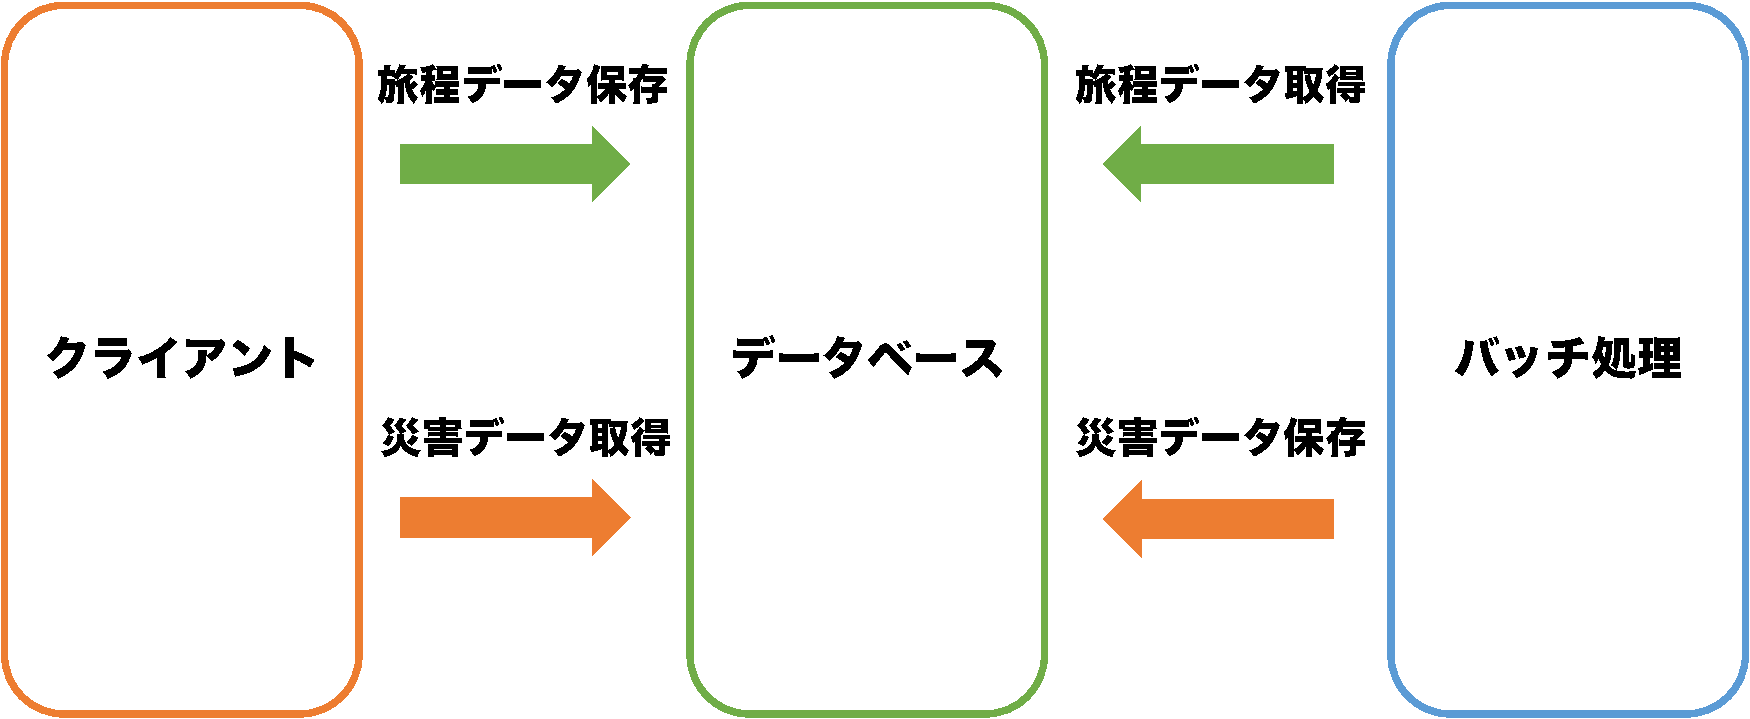
\includegraphics[height=6cm]{figure31.pdf}
  %\vspace{-3mm}
  \caption{システムの全体概要図}
  \label{fig:system_summary}
  %\vspace{2mm}
\end{figure}

\subsection{クライアント部}
クライアント部はこのシステムにおけるユーザインタフェースの役割を持つ.
旅程データの入力機能と注意情報を提供する機能がある.
具体的にはモバイルアプリケーションとして開発した.

\subsubsection{旅程データの入力機能}
ユーザはまず旅程のタイトルと期間を入力し,旅程パッケージを作成する.
旅程パッケージとは旅程データを1つにまとめたものである.
旅程データには,場所データと交通機関のデータの2種類が存在する.ユーザはこの2種類のデータで旅程を構築する.
ユーザは訪れる予定の場所や利用する予定の交通機関の位置情報を,予定時刻とともに入力インタフェースを通して入力する.
位置情報は両方の種類においても都道府県と市区町村名の名称である.
インタフェースは旅程パッケージごとに入力されたデータをデータベースへ保存する.
保存する際には旅程パッケージにクライアントIDを付与する.

\subsubsection{注意情報提供機能}
第1章で定義したストック情報とフロー情報をユーザに提供する.
旅程データの入力機能にて事前に入力した旅程データのうち,災害の影響を受けると判断された旅程データを表示する.
その際に影響を受ける災害の種類と可能性の確率を提供する.
さらに,ユーザに対して災害の種類ごとにその現象と対処法についての情報を提供する.
また,影響を受ける旅程データが交通機関である場合,災害の可能性を交通機関が運休する可能性として情報を提供する.
その際に,運休によって起こる現象についての情報を提供する.

\subsection{データベース部}
データベース部はこのシステムにおけるデータを管理する役割を持つ.
データを保存する機能とデータを提供する機能がある.
具体的にはクラウドデータベースを用いている.

\subsubsection{データ保存機能}
ユーザがクライアント部で入力した旅程データを旅程パッケージごとに保管する.
また,バッチ処理部で旅程データと紐付けられた注意情報も保管する.

\subsubsection{データ提供機能}
クライアント部の要求には,旅程パッケージに付与されているクライアントIDを条件にデータを提供する.
バッチ処理部の要求には,旅程データの予定時刻を条件にデータを提供する.

\subsection{バッチ処理部}
バッチ処理部は,旅程データが災害の影響を受けるか監視する役割を持つ.
気象庁が定期的に公表する,注意情報を取得して,ユーザがクライアント部で入力した旅程データと照合する.
災害の影響を受ける旅程データがあれば注意情報と旅程データを紐づけてデータベースに保存する.
旅程データを作成したクラアントに通知する指示を出す.
具体的にはPythonのプログラムを作成して,定期事項している.

\subsubsection{気象庁から注意情報の取得}
注意情報とは災害の影響を受ける可能性と予定時刻,発表地域で構成される情報である.
この情報は気象庁から定期的にWeb上で発表されている.
その時刻に合わせてバッチ処理が実行され,注意情報を取得する.

\subsubsection{旅程データの取得}
注意情報の予定時刻と重なる旅程データを検索する.
データベース部から旅程データを取得する.

\subsubsection{注意情報と旅程データを照合}
注意情報の予報時刻に当てはまる旅程データを抽出した後,旅程データの場所情報をもとに,注意情報を関連付けて保存するか判断する.
注意情報の発表地区は気象庁が独自に定めている,各都道府県の市区町村のまとまりである.
注意情報に災害の予測が記載されている場合,旅程データの位置情報から発表地区に属するデータを抽出し,注意情報を旅程データと紐付ける.
災害の影響を受けると判断された旅程データはデータベースに保存する.
もし注意情報に災害の予測が記載されてなければ何もしない.


\subsubsection{クライアント部へ通知指示}
災害の影響を受けると判断された旅程データを作成したクライアントに通知を送信するよう指示を出す.
しかし,評価実験をするにあたって評価指標とは関連がない機能であったことと,コスト削減のため本研究ではクライアント部からの通知機能を実装した.

\subsection{処理の流れ}
システムの処理の流れについて述べる.
図 \ref{fig:activity}にアクティビティを示す.

\begin{quote}
  \begin{enumerate}
    \item 旅程データの入力(クライアント部)
    \item 旅程データの保存(データベース部)
    \item 気象庁から注意情報の取得(バッチ処理部)
    \item 旅程データの取得(バッチ処理部)
    \item 旅程データの提供(データベース部)
    \item 注意情報と旅程データを照合(バッチ処理部)
    \item 注意情報の保存(データベース部)
    \item クライアント部へ通知指示(バッチ処理部)
    \item 通知(クライアント部)
    \item 注意情報の提供(データベース部)
    \item 注意情報提供(クライアント部)
  \end{enumerate}
\end{quote}

\begin{figure}[H]
  \centering
  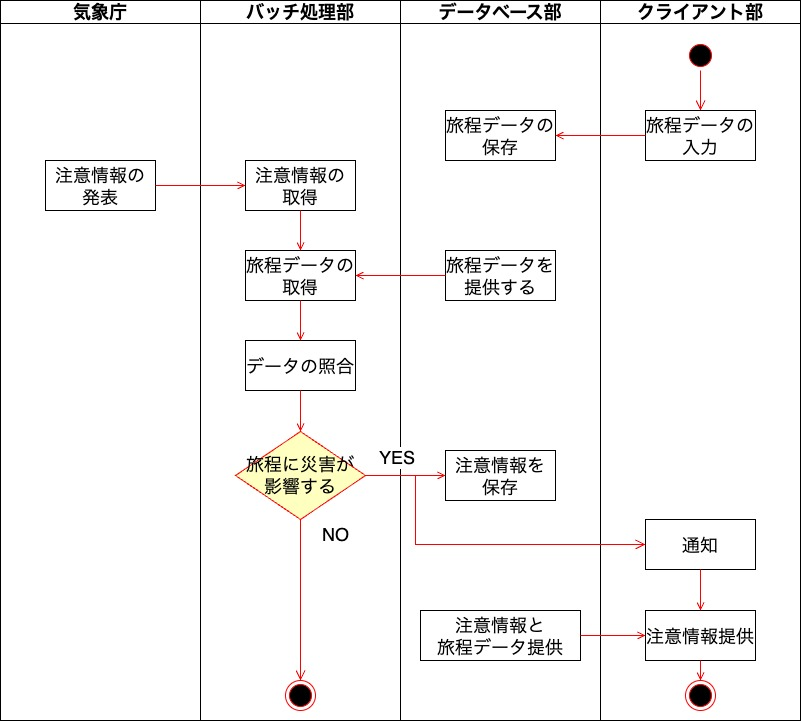
\includegraphics[height=10cm]{figure32.jpg}
  %\vspace{-3mm}
  \caption{システムのアクティビティ図}
  \label{fig:activity}
  %\vspace{2mm}
\end{figure}
\section{ファイル構成}
配布したフォルダには様々なファイルが同梱されているが,拡張子が「tex,bib,cls,bat」であるファイルが重要である.

拡張子が「tex」ファイルは,本文を記載するファイルである.
本文中には,\LaTeX の命令をマークアップしていく.

拡張子が「bib」ファイルは,参考文献を記載するファイルである.
\BibTeX の命令でマークアップしていく.
このファイルを \LaTeX 側から呼び出し,参照したり番号を割り振ったりする.

拡張子が「cls」ファイルは,設定事項を記載するファイルである.
基本的に,この拡張子のファイルは変更する必要は無い.

拡張子が「bat」ファイルは,\LaTeX のソースファイルから,PDFファイルを作成するまでの一連の命令を実行するバッチファイルである.
\LaTeX において標準的には,本バッチファイル内の命令は各自で順に実行するのだが,煩雑である.
宮治が作成した(というほどのものではないが)本バッチファイルを実行すれば,その中の命令は意識する必要はない.
今回配布のバッチファイルは Macintosh と Windowsで別のものを利用する.

主要なファイルの説明を 表\ref{table:files2}に記載する.
\begin{table}[H]
\centering
\caption{スタイルパッケージ内のファイル説明}
\vspace{-2mm}
{\footnotesize
\begin{tabular}{|l|l|l|}
\hline
ファイル名 & 内容 & 注意\\\hline\hline
settings.tex & 論文の必要事項設定ファイル & 必ず編集\\\hline
main.tex & 大元のファイル & 読み込むファイルなどを設定\\\hline
main.dvi & できたファイル & \\\hline
main.pdf & pdfファイル & dvi ファイルを元に作成\\\hline
myjlab.sty & 宮治研用スタイルファイル & 変更不要\\\hline
myjlabthesisstyle.sty & 各種スタイルファイルを読み込む & 必要に応じて追加\\\hline
abstract.tex & 要旨を記述 & 章や節の命令は入れずに文章を入力\\\hline
thanks.tex & 謝辞を記述 & 章や節の命令は入れずに文章を入力\\\hline
chap1.tex & 第1章を記述 & \\\hline
chap2.tex & 第2章を記述 & \\\hline
sec21.tex, sec22.tex など& 2章1節と2節のファイル & chap2.texが大きくなったのでファイルを分割\\\hline
chap3.tex & 第3章を記述 & 注:3章内のファイルも節毎にファイルを分割\\\hline
chap4から6.tex & 4章から6章のファイル & 配布無し,各自で作成し,main.tex修正\\\hline
appendixa.tex & 付録Aを記述 & \\\hline
appendixb.tex & 付録Bのファイル & 配布無し,各自で作成し,main.tex修正\\\hline
myrefs.bib & 参考文献情報ファイル & 記述方法が特殊\\\hline
mklatex.bat & Macintosh用の実行バッチファイル & 命令を憶えずとも,main.tex⇒main.pdf\\\hline
winmklatex.bat & Windows用の実行バッチファイル & 命令を憶えずとも,
main.tex⇒main.pdf\\\hline
dmklatex.bat & Docker用の実行バッチファイル & 命令を憶えずとも,
main.tex⇒main.pdf\\\hline
\end{tabular}
}
\label{table:files2}
\end{table}

これらのファイルの変更方法,記入方法を以降で解説する.
\section{settings.tex: 論文の設定情報を記述}
settings.tex には,各自の個人情報や論文のタイトルなどを設定する.

\subsection{各自の情報設定}
各自の情報を設定する際には,サブタイトルの有り/無しで設定事項が異なることに注意をする必要がある.
それぞれの方法について以下に記述する.
また,これらの作業が終わった時点で,本配布スタイルパッケージの動作確認をすることをおすすめする.

\subsubsection{サブタイトル有りの場合}
配布したファイルは,サブタイトルがある場合のサンプルになっている.
各自の 年度,提出年月,学籍番号,氏名,タイトル,サブタイトルを所定の命令内に記入する.
\begin{breakbox}
{\small
%footnotesize
\begin{verbatim}
\nendo{2013年度}
\teisyutsu{2014年~~1月}
\snum{15387019}
\jname{宮治 裕}
\thesistitle{宮治研における論文作成について} %タイトルを記入
\thesissubtitle{\LaTeX の利用} %サブタイトルを記入 ない場合はコメントアウト
\SUBTtrue %サブタイトル有りの場合 ない場合は,コメントアウト
%\SUBTfalse %サブタイトル無しの場合 有る場合は,コメントアウト
\end{verbatim}
}
\end{breakbox}

\subsubsection{サブタイトル無しの場合}
サブタイトル有りの場合と比較して2箇所の変更が必要である.
サブタイトルを記入する命令の先頭部分に \% 記号を入れ,コメントアウト状態にする.

\begin{breakbox}
{\small
\begin{verbatim}
%\thesissubtitle{\LaTeX の利用} %サブタイトルを記入 無い場合は,コメントアウト
\end{verbatim}
}
\end{breakbox}
もう一つは,その直下の2行
\begin{breakbox}
{\small
\begin{verbatim}
\SUBTtrue %サブタイトル有りの場合 無い場合は,コメントアウト
%\SUBTfalse %サブタイトル無しの場合 有る場合は,コメントアウト
\end{verbatim}
}
\end{breakbox}
以下の様に変更する.
\begin{breakbox}
{\small
\begin{verbatim}
%\SUBTtrue %サブタイトル有りの場合 無い場合は,コメントアウト
\SUBTfalse %サブタイトル無しの場合 有る場合は,コメントアウト
\end{verbatim}
}
\end{breakbox}

以上の設定で,表紙と各ページのヘッダ・フッタの情報が自動的に設定され,書式が整えられる.
\begin{boxnote}
\LaTeX では 「\verb+%+」はコメントを意味し,この記号から改行コードまでをコメントアウト状態として処理する.
\end{boxnote}
であることに注意すること.

\subsection{スタイルパッケージの動作確認}
サブタイトルの有り/無しに応じて適切に設定ができた段階で,一度各自の環境下でスタイルパッケージが正常動作することを確認して欲しい.
正常動作した場合には,本ファイルとほぼ同様の中身で,表紙と各ページのヘッダとフッタが各自の設定した情報が記載されたPDFファイルが出来上がるはずである.

まず,Macintoshの場合について記す.
各自のホームディレクトリ中のDropboxフォルダ内に,本スタイルパッケージが展開されている場合を前提として記述する.
\begin{enumerate}
\item まず,ターミナルを開く
\item 以下のコマンドを入力し,スタイルパッケージのあるフォルダに移動
\footnote{ここで \verb+$+記号は,コマンドプロンプトを表すため,入力しないように.}
\begin{screen}
{\small
\begin{verbatim}
 $ cd ~/Dropbox/Thesis
\end{verbatim}
}
\end{screen}

\item そこで,バッチファイル \verb+mklatex.bat+ を実行
\begin{screen}
{\small
\begin{verbatim}
 $ ./mklatex.bat
\end{verbatim}
}
\end{screen}

\item main.pdfファイルが作成され,プレビュー画面が自動で表示される
\item[\textbf{注}] mklatex.bat が実行できないというようなエラーが出た場合には,最初の一回だけ(次回から不要)以下の命令を入力する
\begin{screen}
{\small
\begin{verbatim}
 $ chmod 755 ./mklatex.bat
\end{verbatim}
}
\end{screen}
\end{enumerate}

正常動作しなかった場合には,出来上がった main.log ファイルを宮治に送付して欲しい.

Windowsの場合には,コマンドプロンプトを開き,目的のフォルダに移動し,バッチファイル(winmklatex.bat)を起動する.
\begin{screen}
{\small
\begin{verbatim}
 $ cd c:\My Documents\Dropbox\Thesis
 $ winmklatex.bat
\end{verbatim}
}
\end{screen}
main.pdfファイルができるので,エクスプローラからファイルをダブルクリックしてAcrobat Reader にて確認して欲しい.

\section{使用方法}

本研究のシステムの使用方法を述べる.使用手順は以下の通りである.

\begin{quote}
  \begin{enumerate}
    \item アプリを起動する
    \item 旅程パッケージを作成する
    \item 旅程データを作成する
    \item 通知を受け取る
    \item 災害注意予報を確認する
    \item ストック情報を確認する
  \end{enumerate}
\end{quote}

\subsection{アプリを起動する}
アプリを利用するのに,旅行計画の作成が必要であるため,機能メニューの旅行計画をタップする.
ホーム画面はアプリを立ち上げたとき,最初に表示される画面である.
この画面ではアプリの概要について説明が閲覧できる.
この画面から予報についての画面と旅程パッケージの作成画面に遷移できる.

\begin{figure}[H]
  \centering
  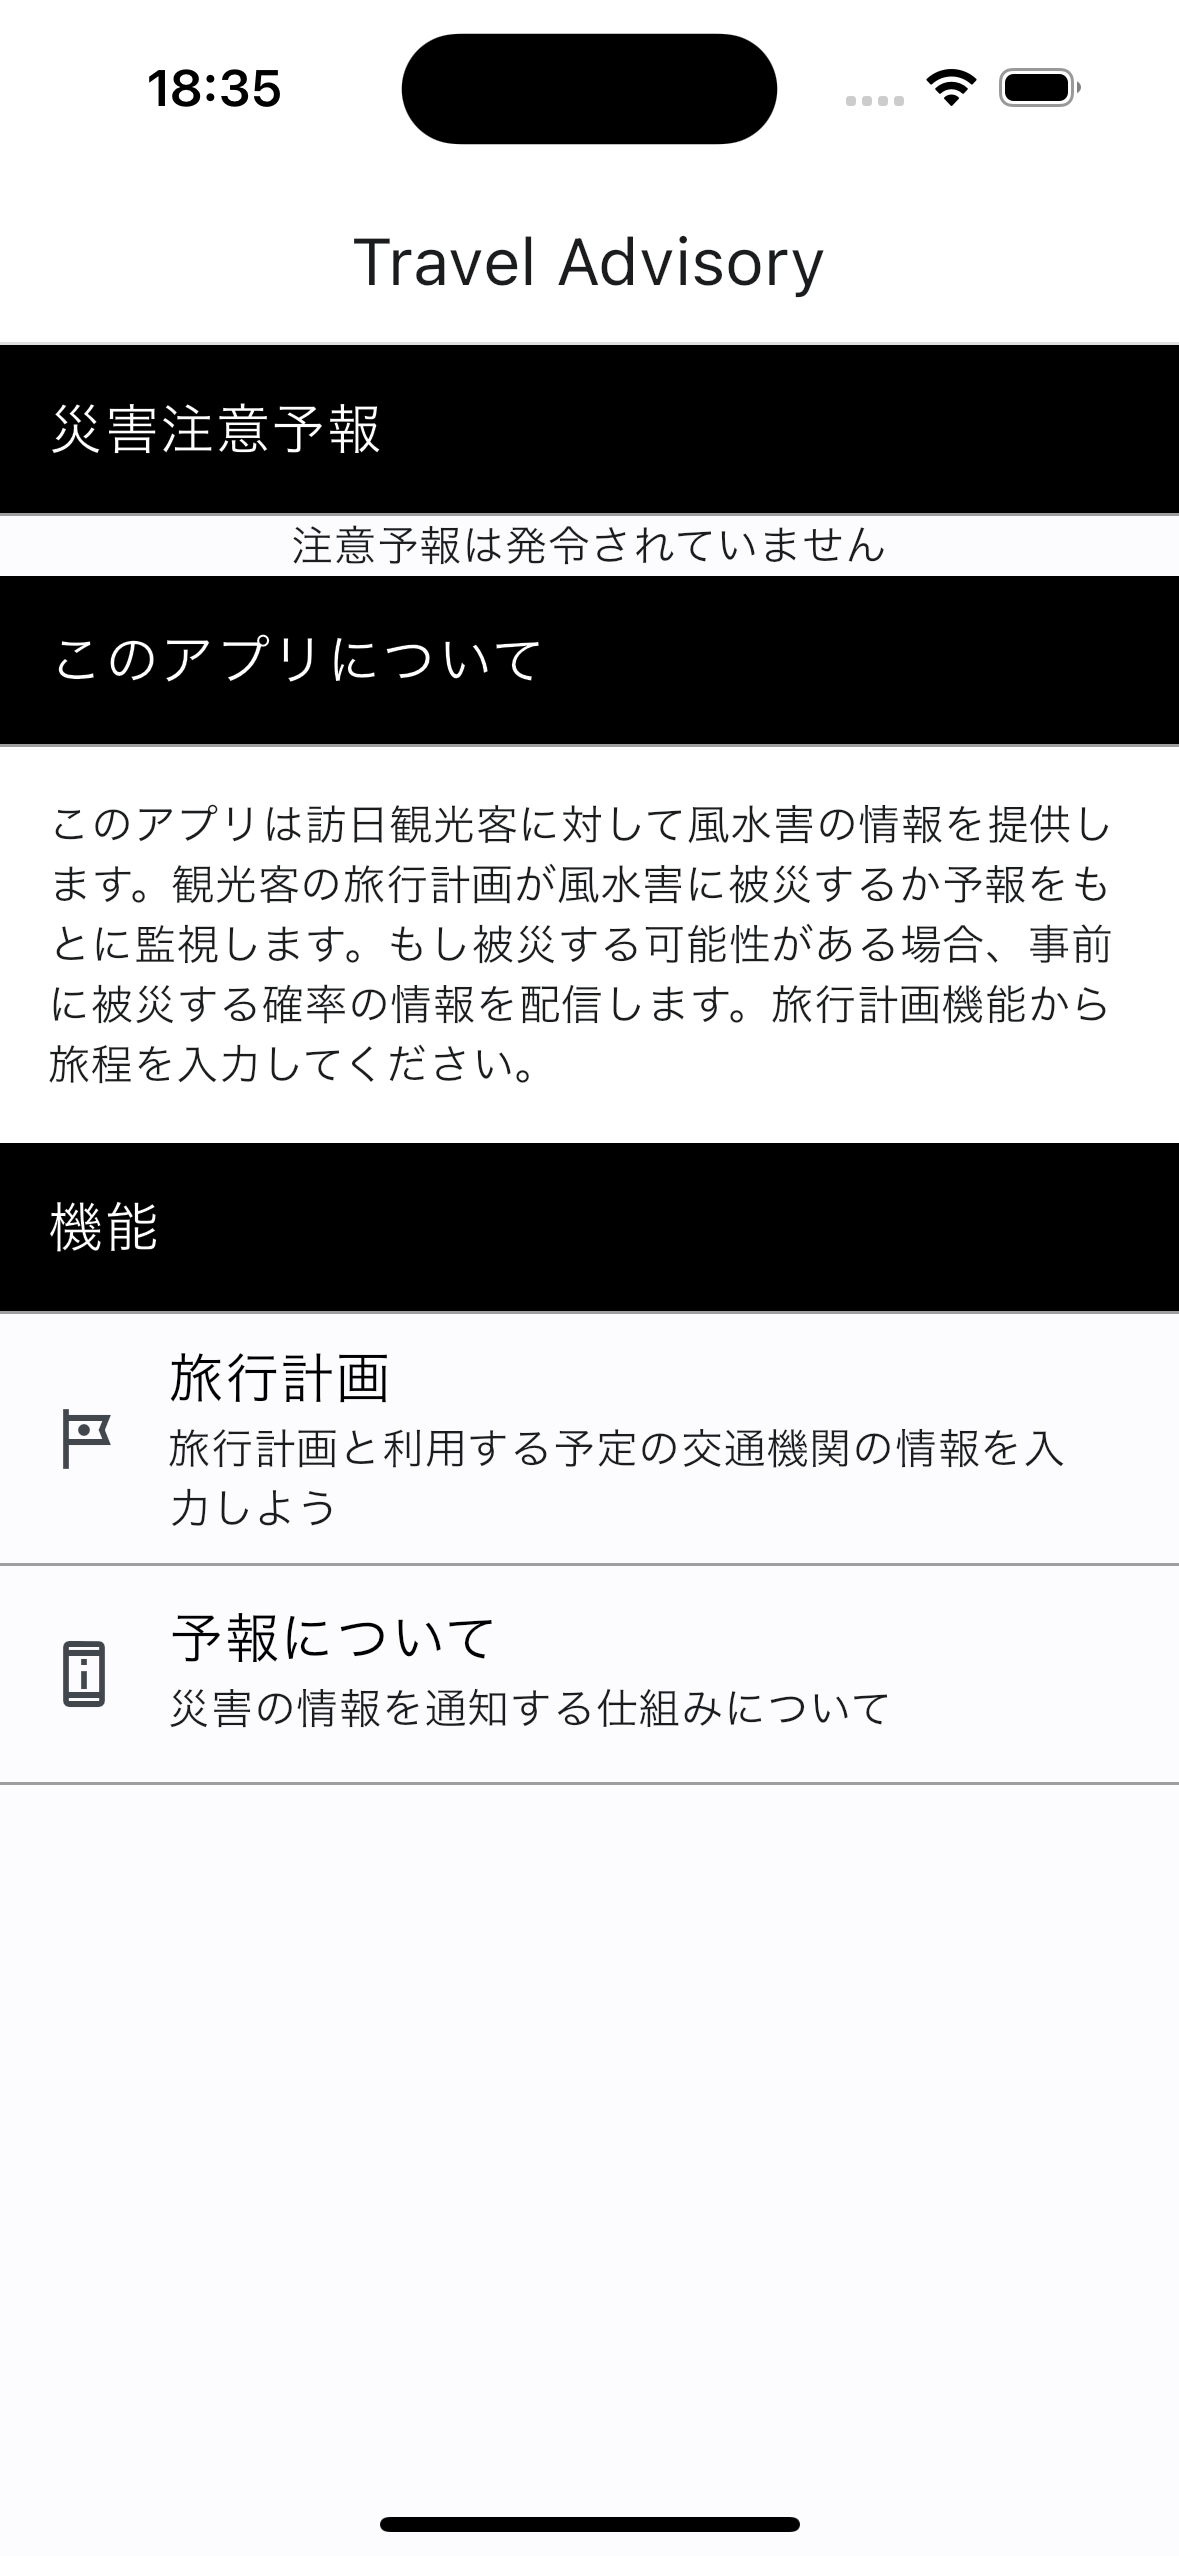
\includegraphics[height=10cm]{./fig/normal_home_screen.png}
  %\vspace{-3mm}
  \caption{通常時のホーム画面}
  \label{fig:normal_home_screen}
  %\vspace{2mm}
\end{figure}

% \subsection{予報についての画面}
% 予報についての画面はアプリケーションが提供する災害注意予報について説明している画面である。
% アプリでの予報の表示の仕方や、気象庁防災情報XMLについて簡単に説明している。

% \begin{figure}[H]
%   \centering
%   \includegraphics[height=8cm]{./fig/forcast_screen_1.png}
%   %\vspace{-3mm}
%   \caption{予報についての画面の図1}
%   \label{fig:forecast_screen_1}
%   %\vspace{2mm}
% \end{figure}

% \begin{figure}[H]
%   \centering
%   \includegraphics[height=8cm]{./fig/forcast_screen_2.png}
%   %\vspace{-3mm}
%   \caption{予報についての画面の図2}
%   \label{fig:forecast_screen_2}
%   %\vspace{2mm}
% \end{figure}

\subsection {旅程パッケージを作成する}
旅程データを作成するために旅程パッケージを作成する.
旅程パッケージ画面は作成した旅程パッケージの一覧と旅行パッケージの作成機能を提供している画面である.
旅行パッケージは右下の計画の作成ボタンをタップすると旅行パッケージ作成画面に遷移して作成できる.
旅行パッケージの一覧からパッケージをタップすると,旅程データ画面に遷移する.

\begin{figure}[H]
  \begin{minipage}[b]{0.45\linewidth}
    \centering
    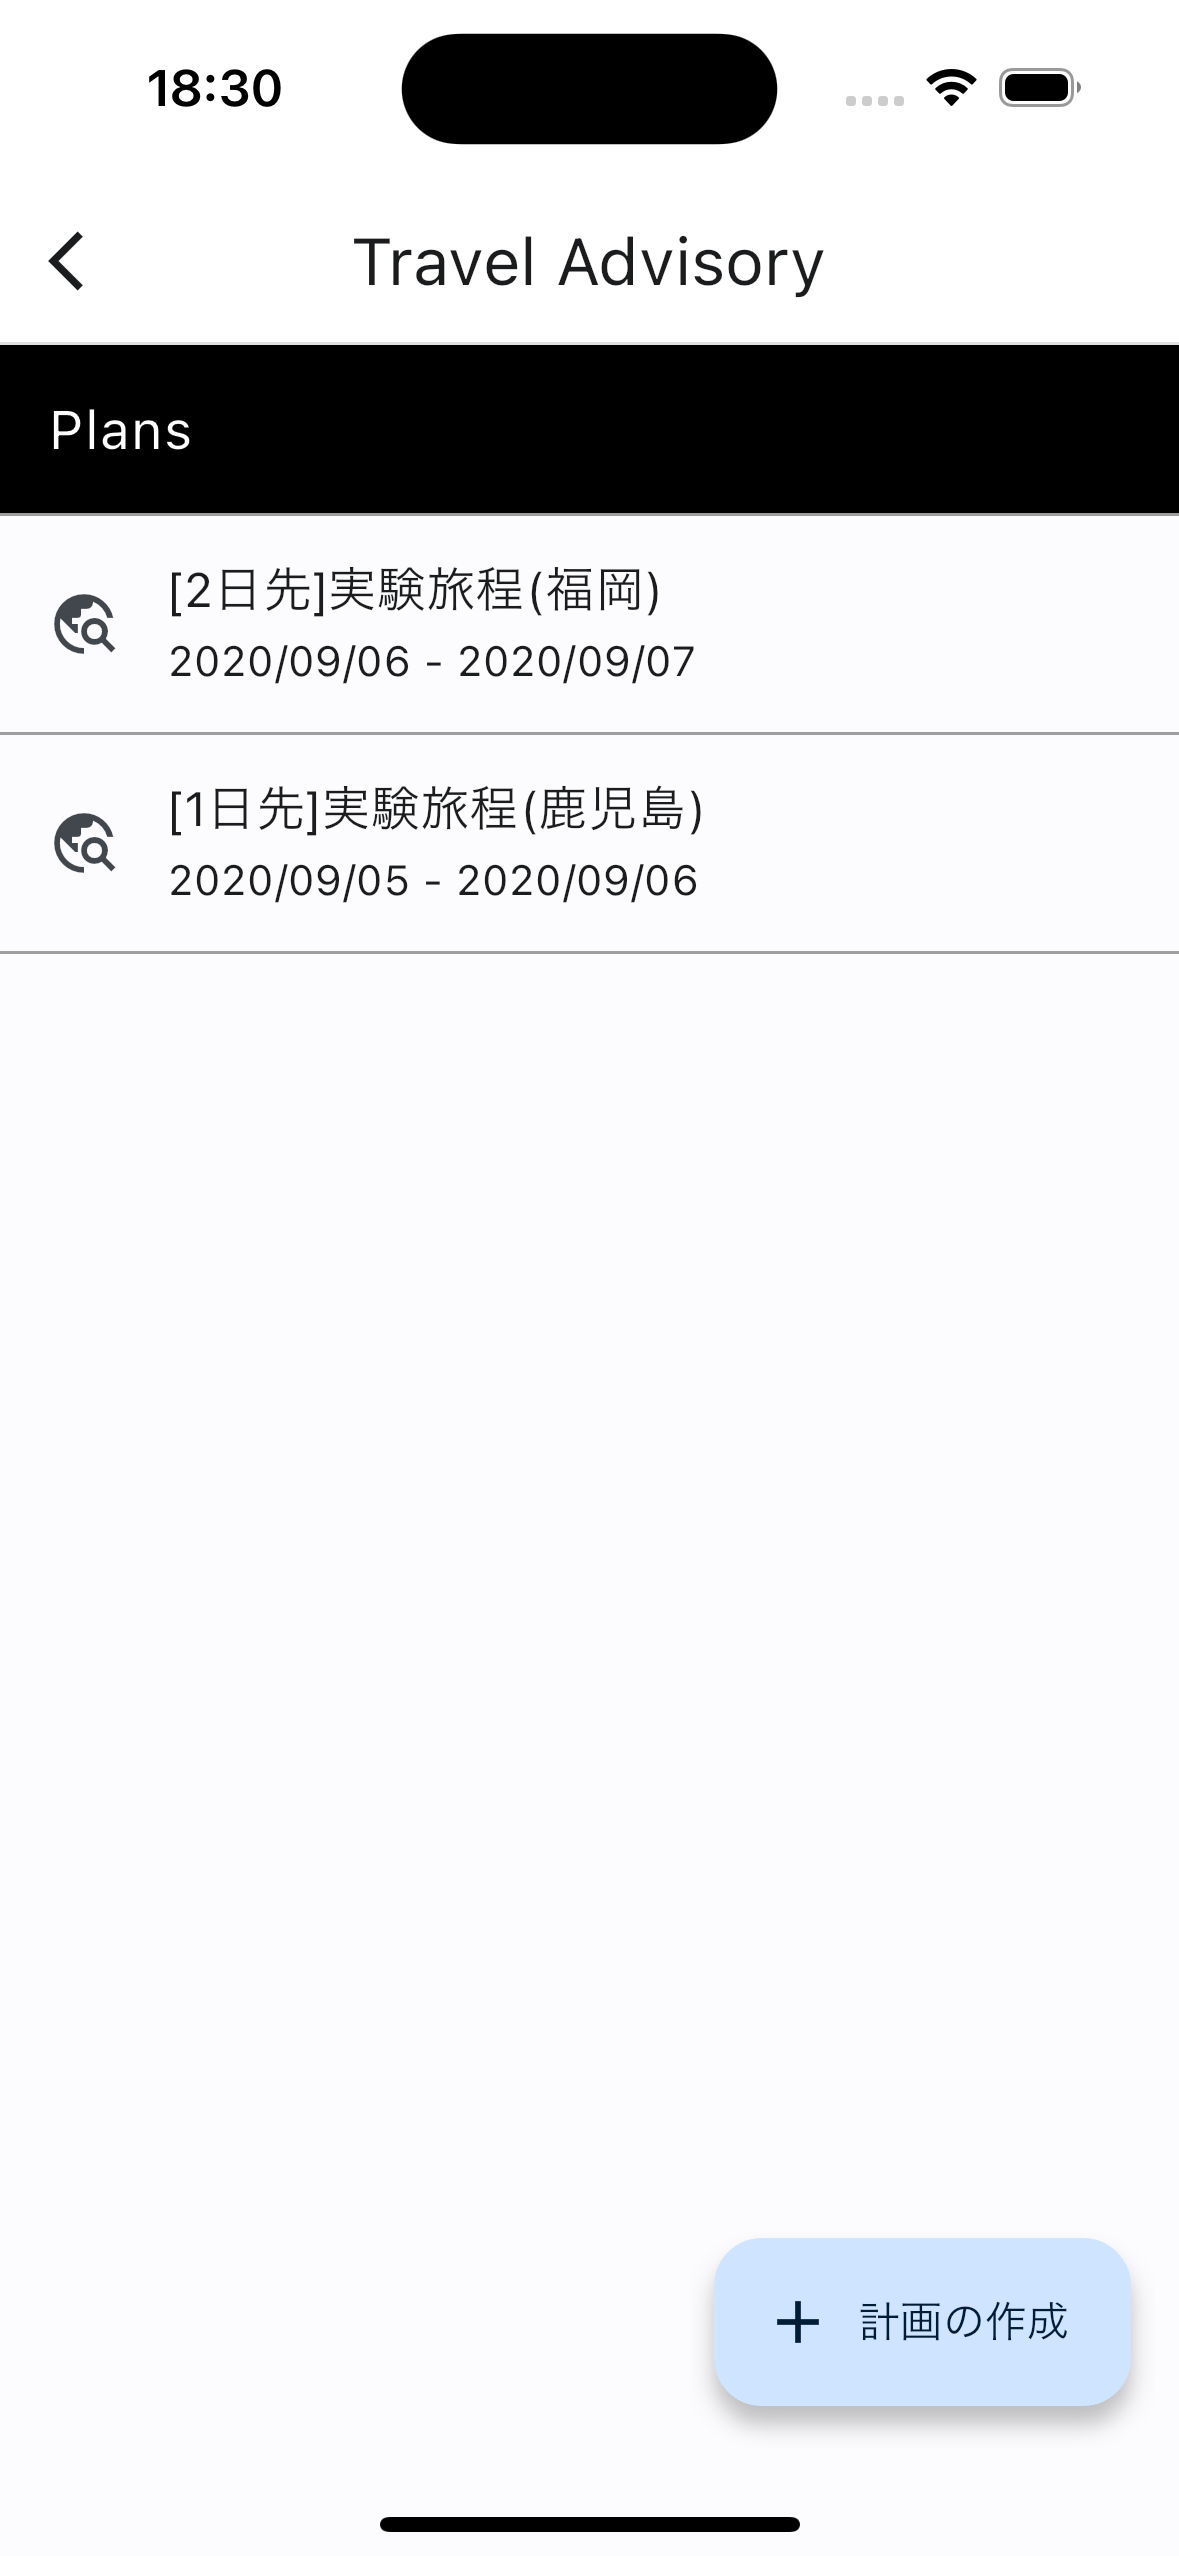
\includegraphics[height=10cm]{./fig/travel_pack_list.png}
    %\vspace{-3mm}
    \caption{旅程パッケージ画面}
    \label{fig:travel_pack_list}
    %\vspace{2mm}
  \end{minipage}
  \begin{minipage}[b]{0.45\linewidth}
    \centering
    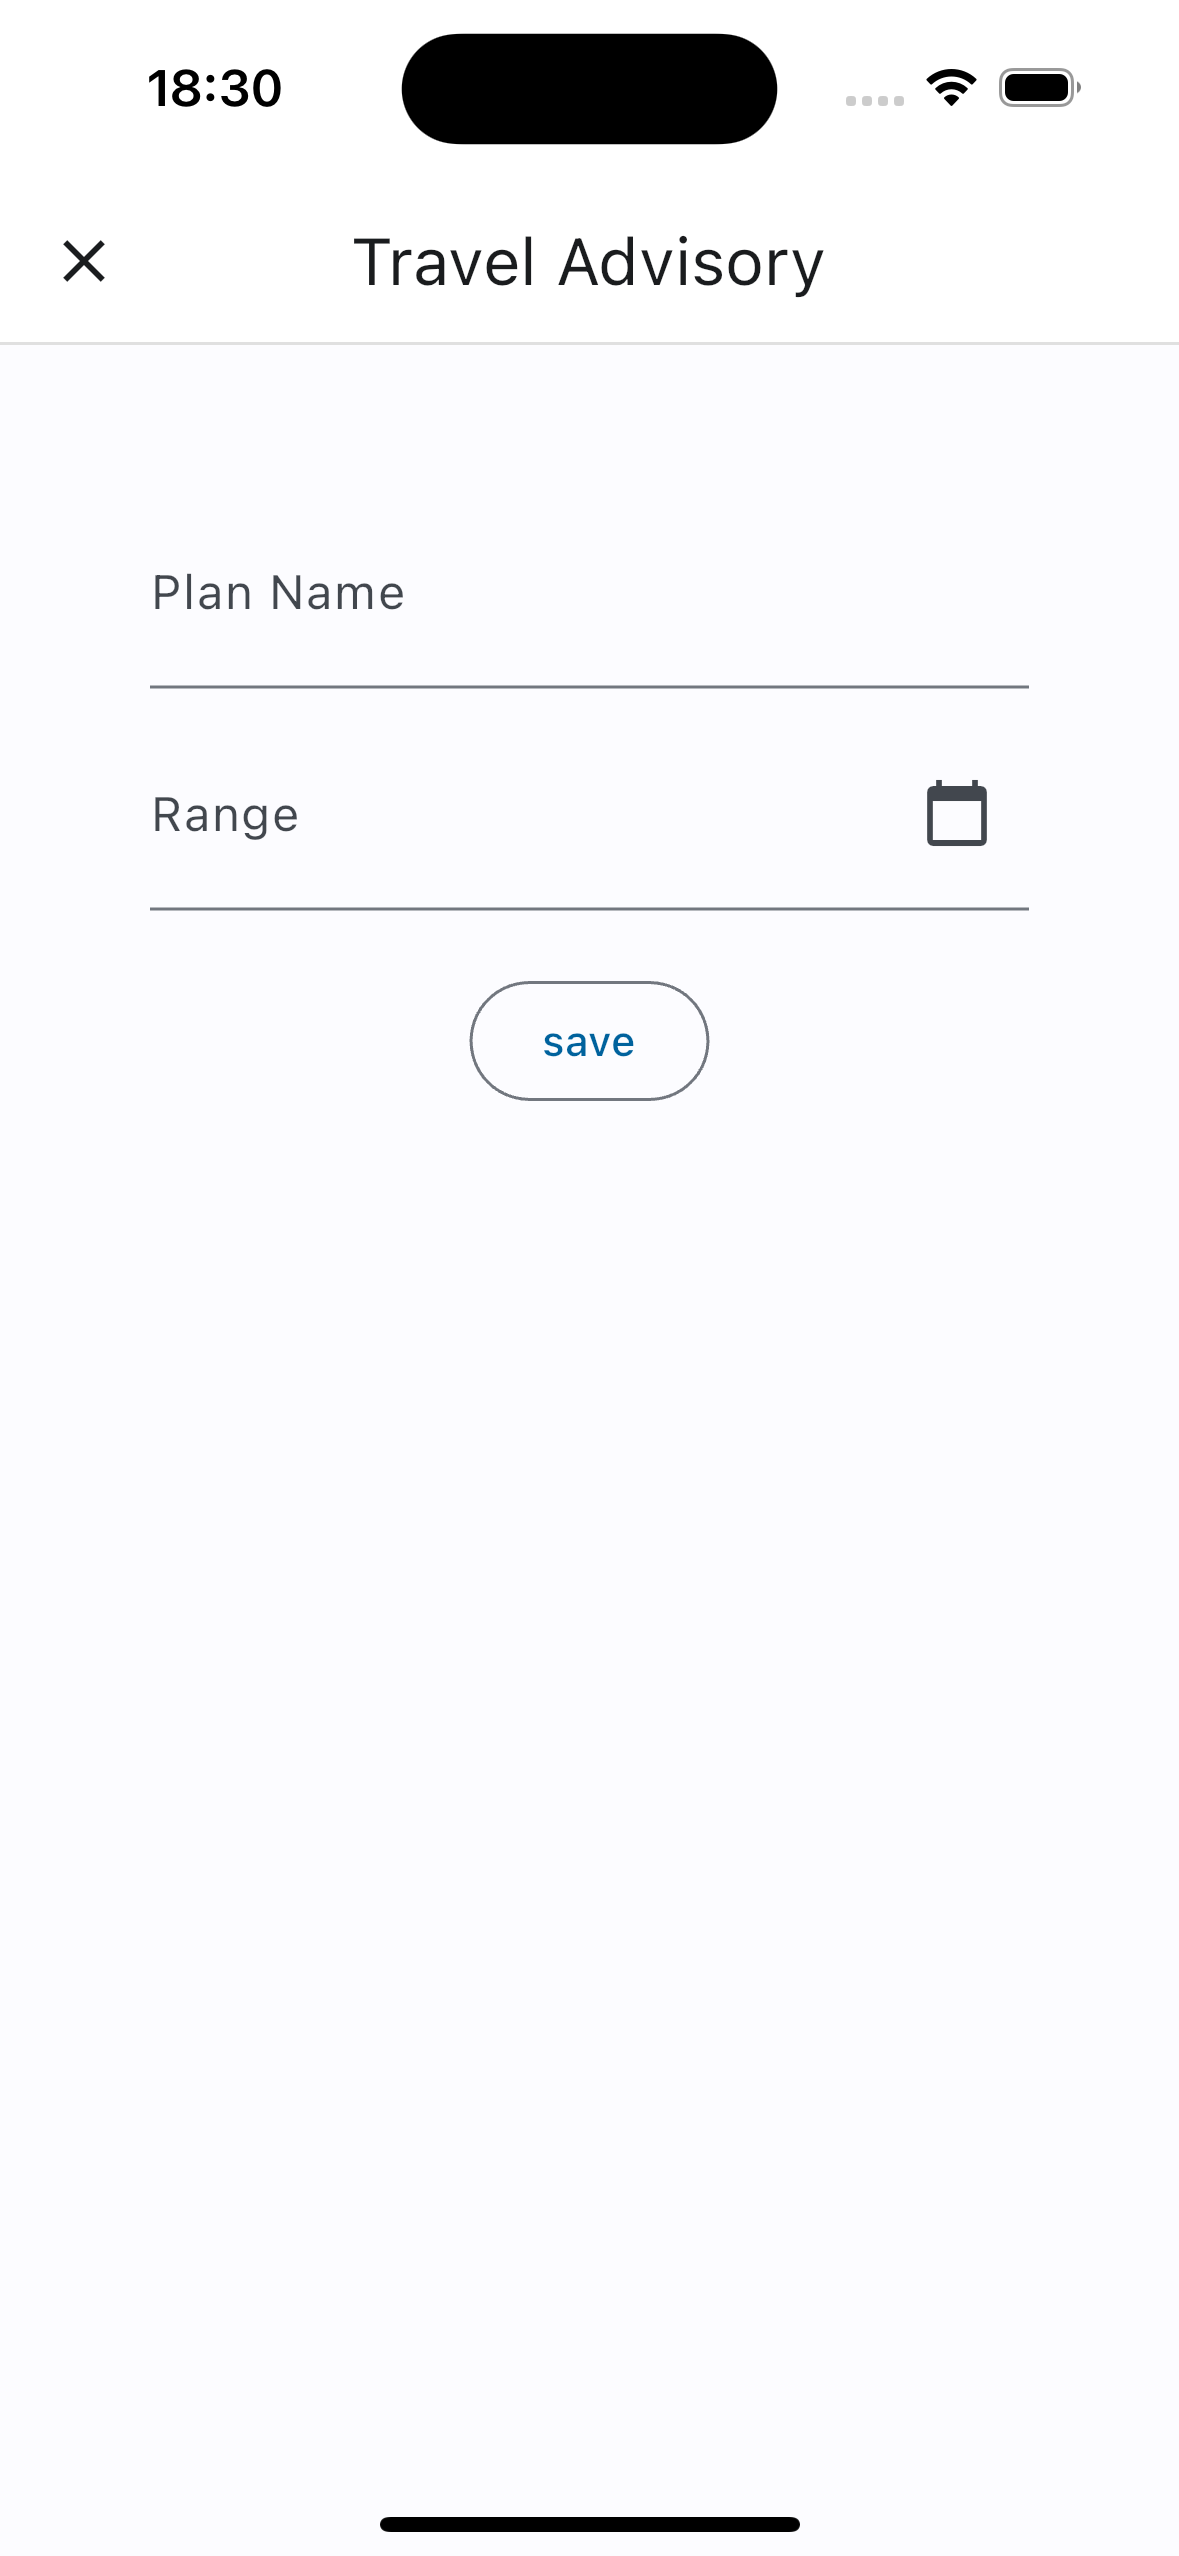
\includegraphics[height=10cm]{./fig/travel_pack_create.png}
    %\vspace{-3mm}
    \caption{旅程パッケージ作成画面}
    \label{fig:travel_pack_create}
    %\vspace{2mm}
  \end{minipage}
\end{figure}

\subsection {旅程データを作成する}
旅程パッケージに旅程データを作成し,登録する.
旅程データ画面は日付ごとに作成した旅程データの一覧と場所・交通データの作成機能を提供している画面である.
下部のAdd Spotボタンをタップすると場所データの作成が,Add Transportationボタンをタップすると交通データの作成画面に遷移する.

\begin{figure}[H]
  \centering
  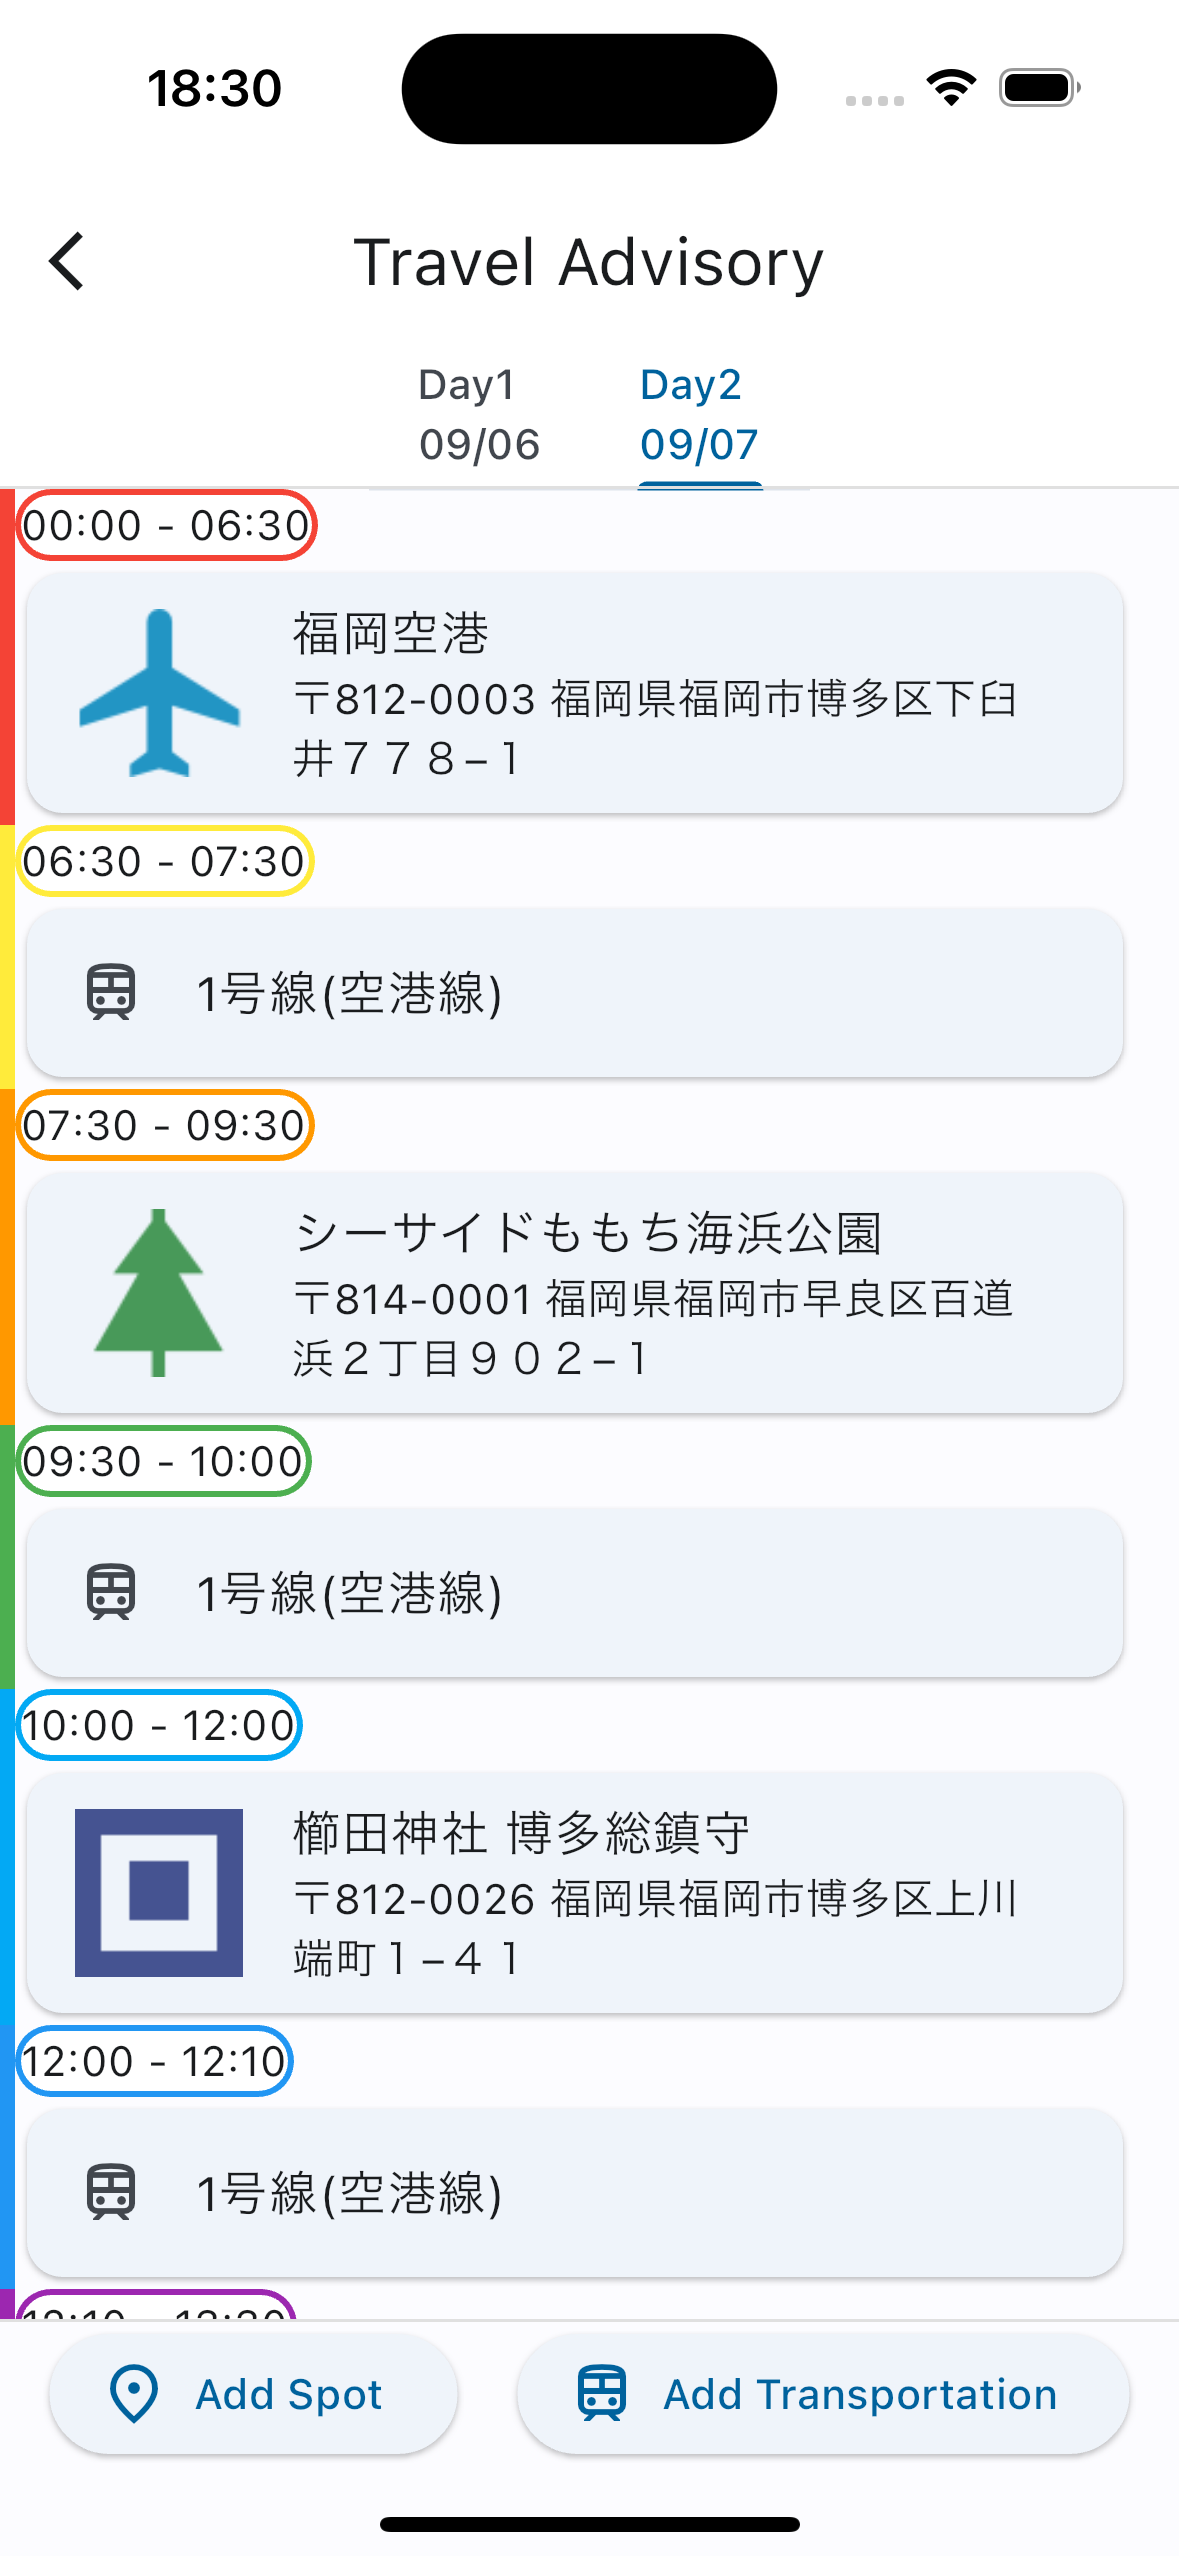
\includegraphics[height=10cm]{./fig/travel_data_list.png}
  %\vspace{-3mm}
  \caption{旅程データ画面}
  \label{fig:travel_data_list}
  %\vspace{2mm}
\end{figure}

\subsubsection {場所データの作成}
場所データを作成する.
訪れる予定の場所を検索する機能とその時刻を入力する機能を提供している画面である.
検索機能はGoogle Map Apiを利用している.
検索すると場所の候補が複数表示されるので,1つを選択してSaveボタンを押す.

\begin{figure}[H]
  \centering
  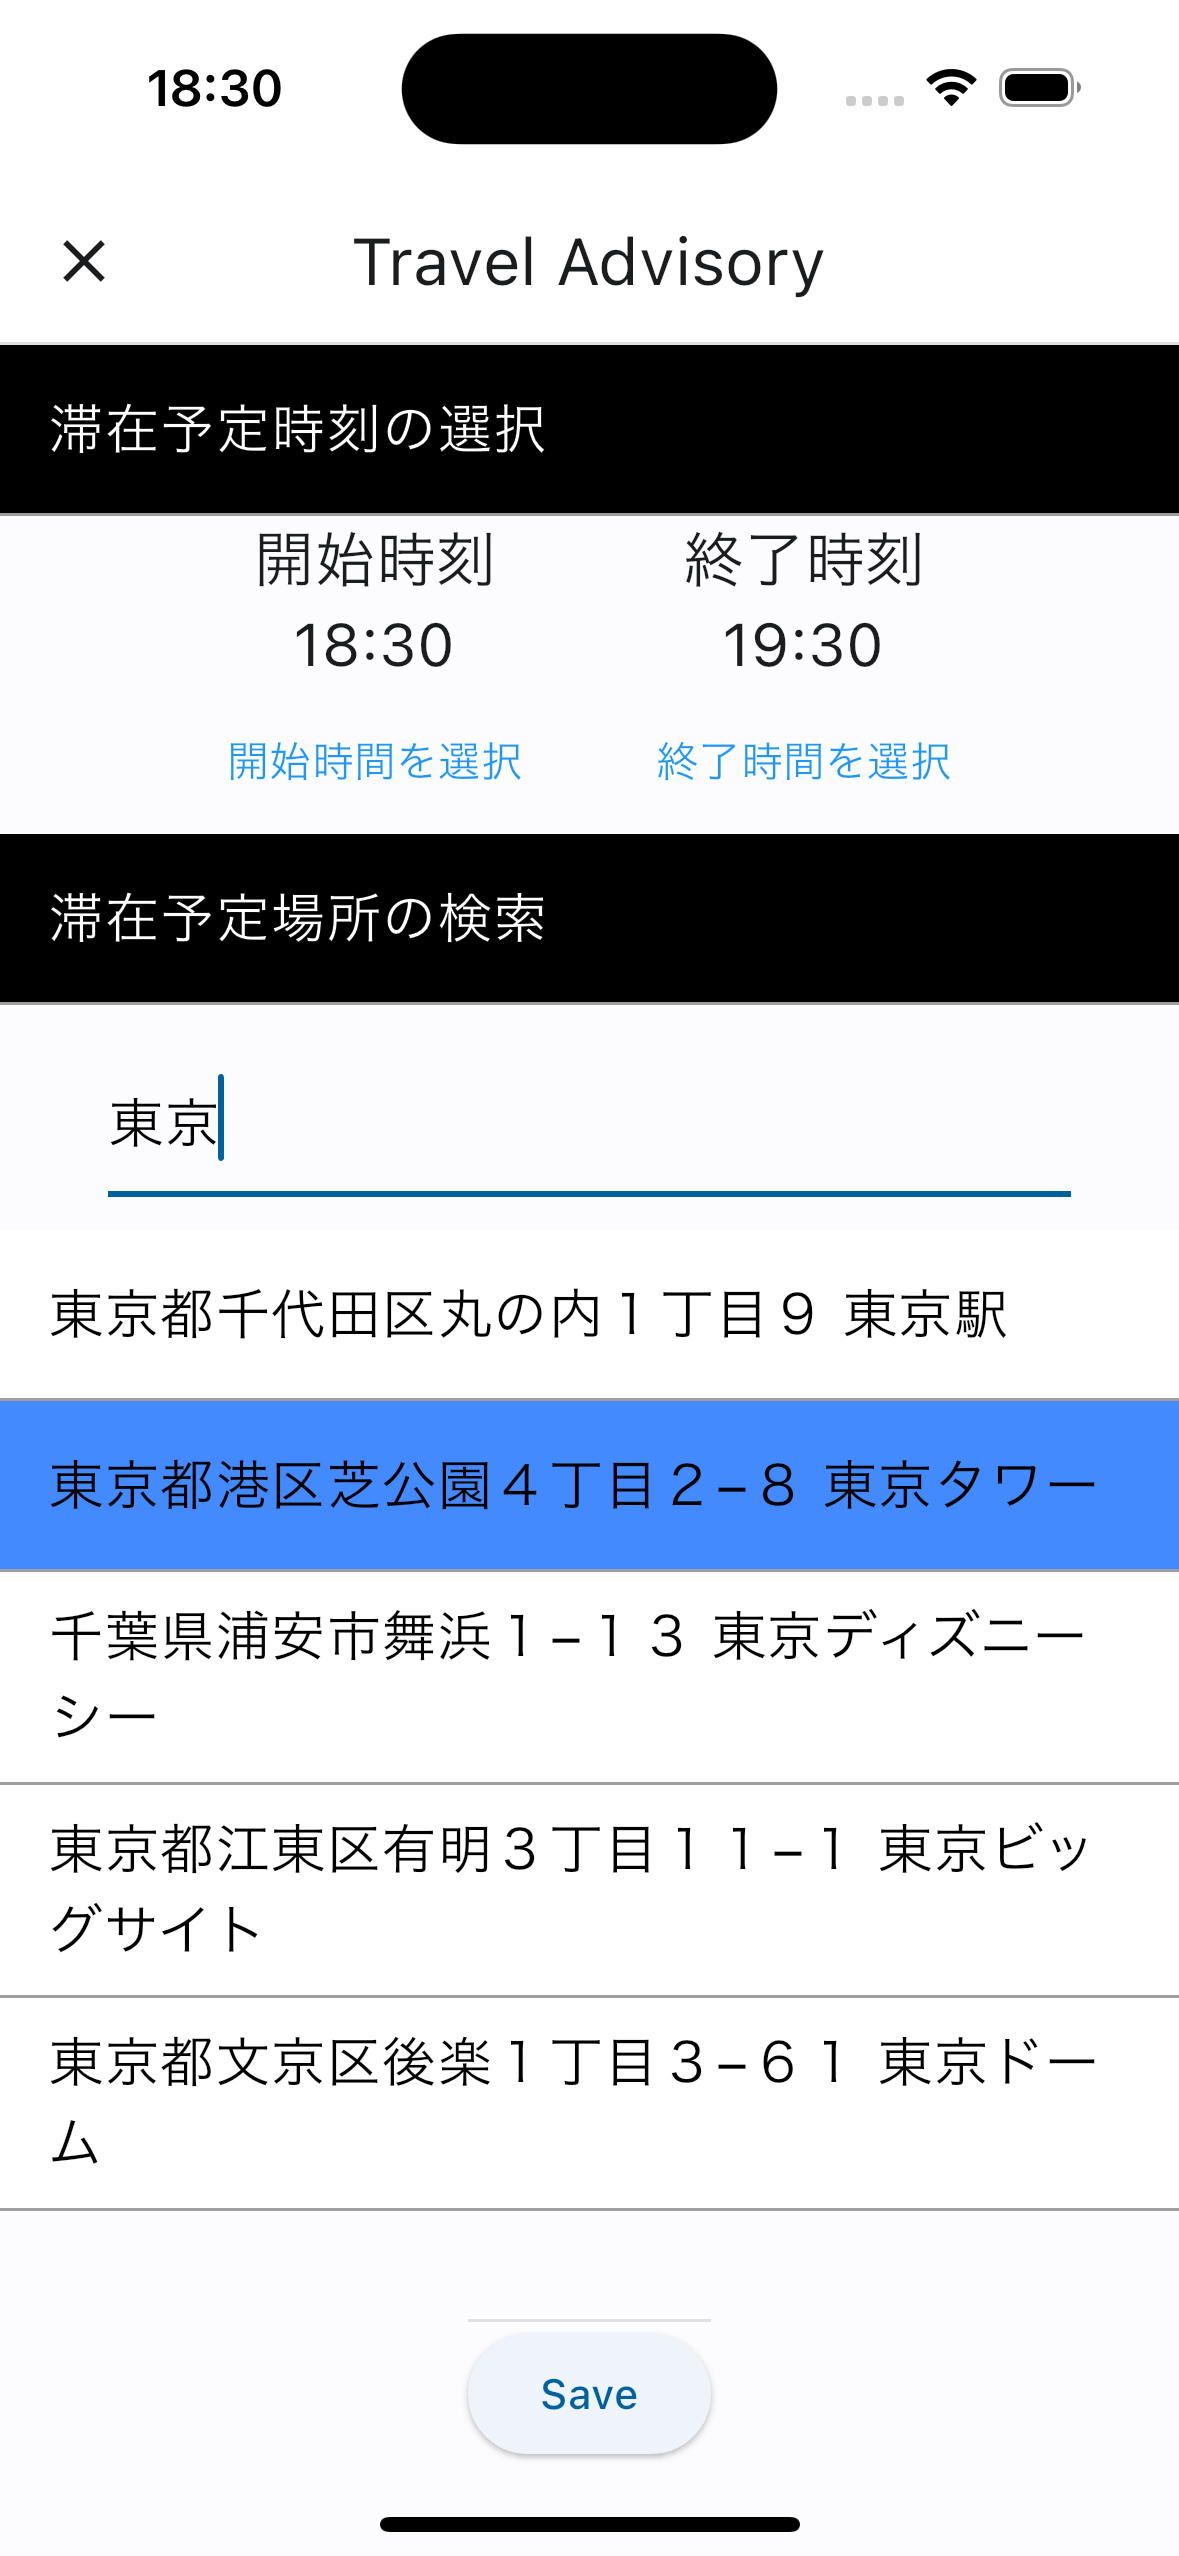
\includegraphics[height=10cm]{./fig/spot_data_save.png}
  %\vspace{-3mm}
  \caption{場所データの作成画面}
  \label{fig:spot_data_save}
  %\vspace{2mm}
\end{figure}

\subsubsection {交通機関データの作成}
交通データを作成する.
利用する予定の鉄道の路線を検索する機能を提供する.
路線を選択した後,路線に属する駅の一覧が表示される.
自分が利用する予定の駅を1つ以上選択し,時刻とともにデータを保存する.

\begin{figure}[H]
  \begin{minipage}[b]{0.45\linewidth}
    \centering
    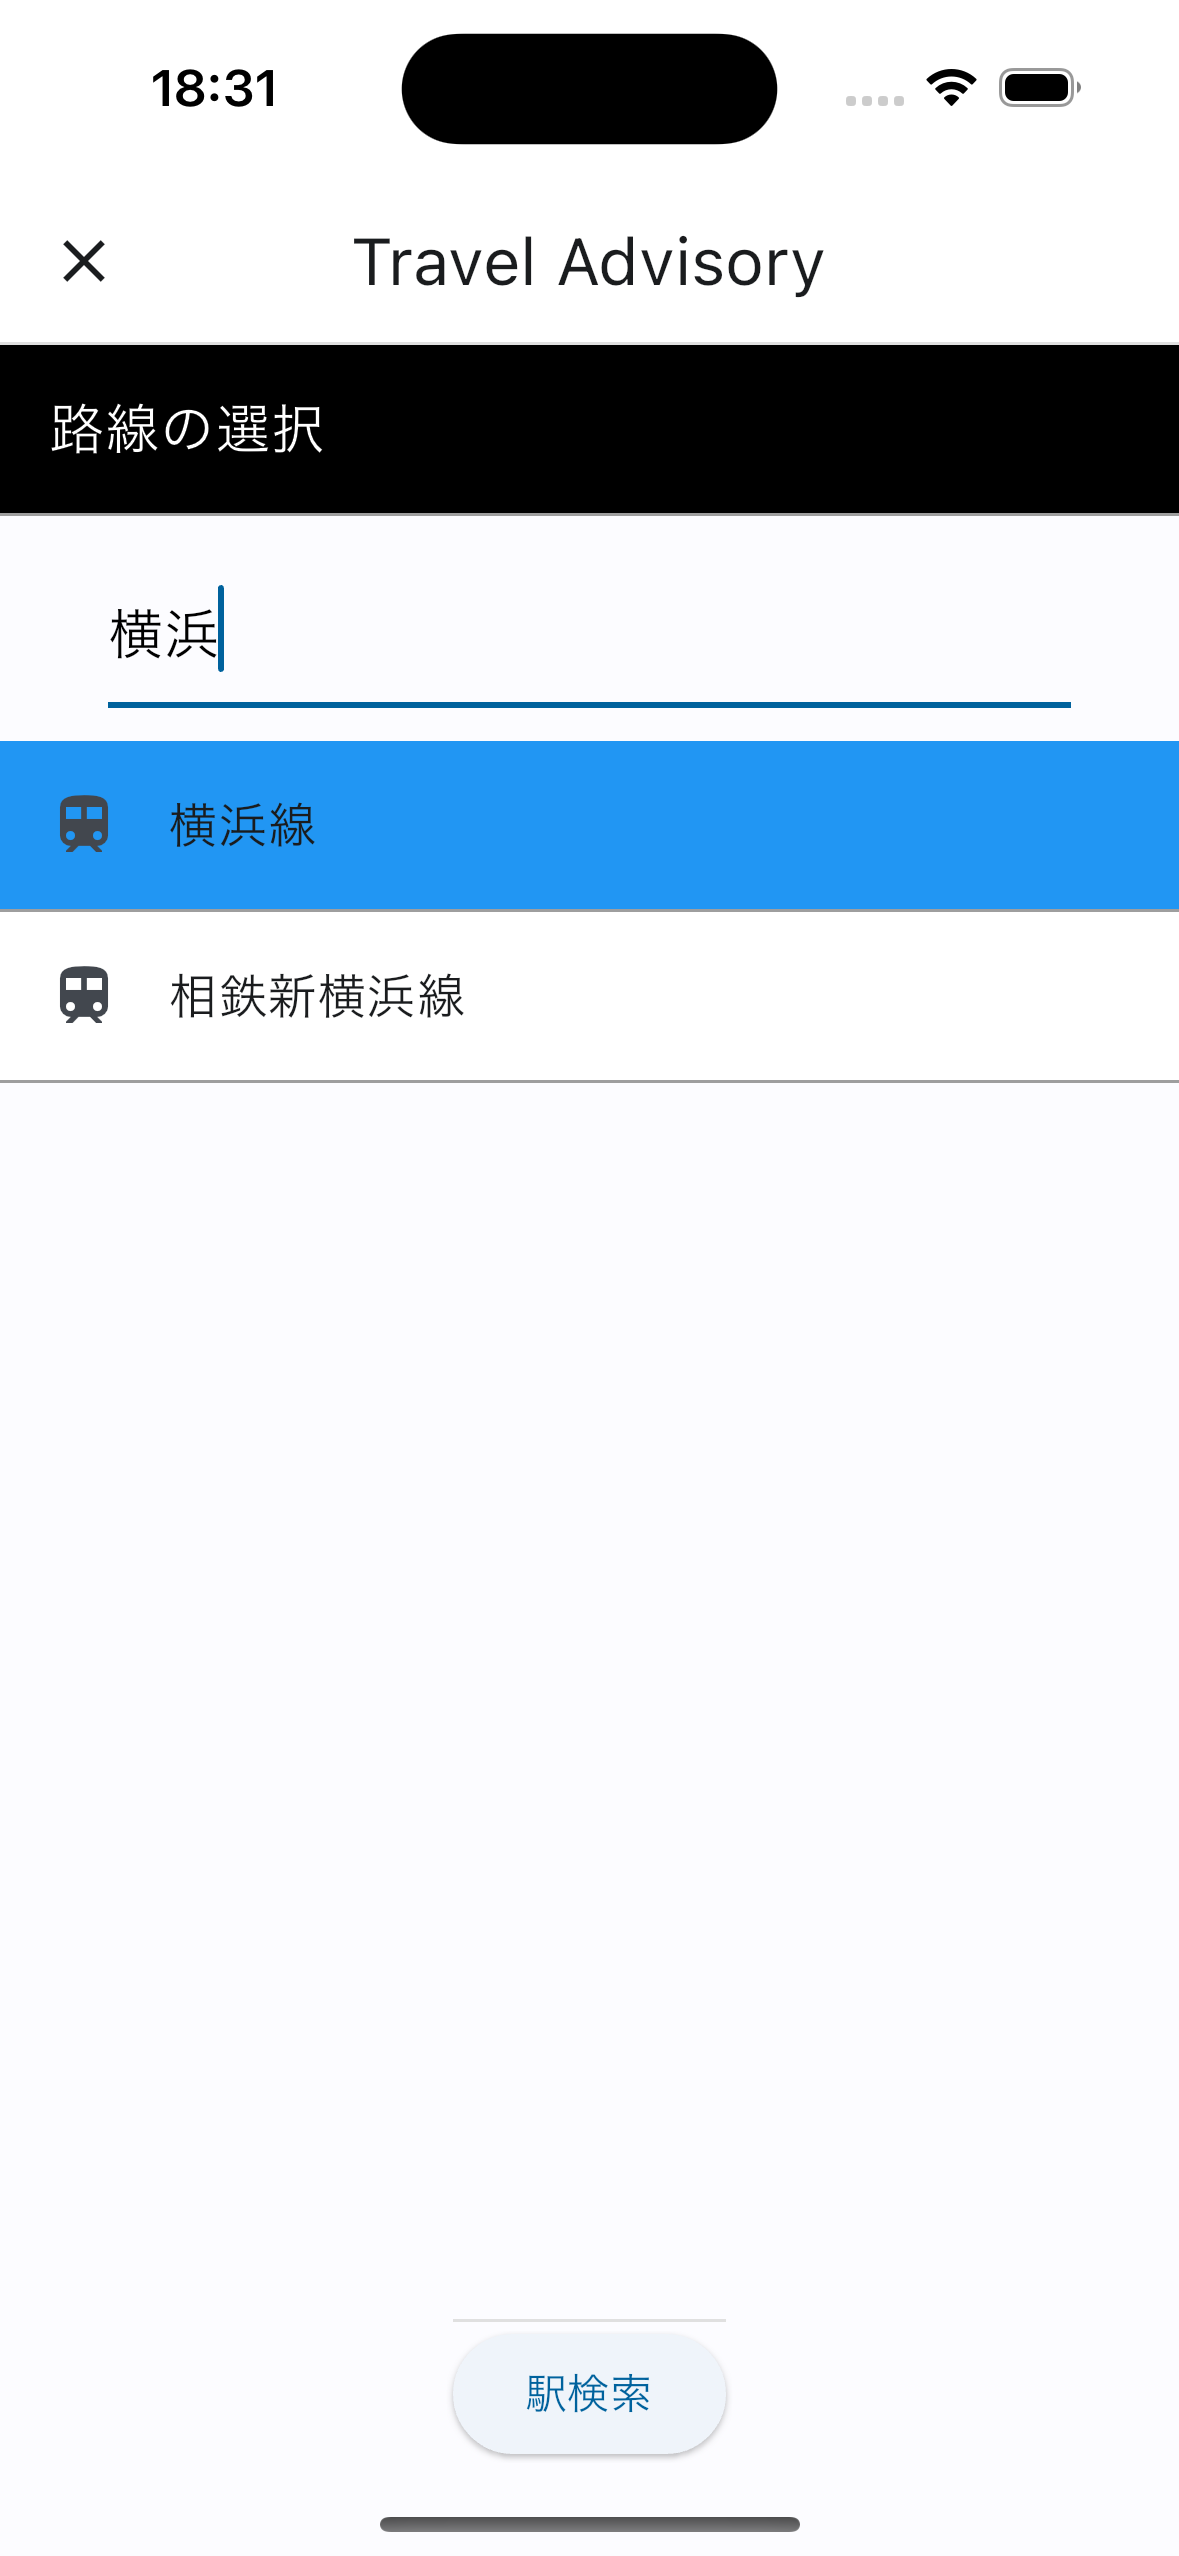
\includegraphics[height=10cm]{./fig/railway_search.png}
    %\vspace{-3mm}
    \caption{鉄道の路線を検索する画面}
    \label{fig:railway_search}
    %\vspace{2mm}
  \end{minipage}
  \begin{minipage}[b]{0.45\linewidth}
    \centering
    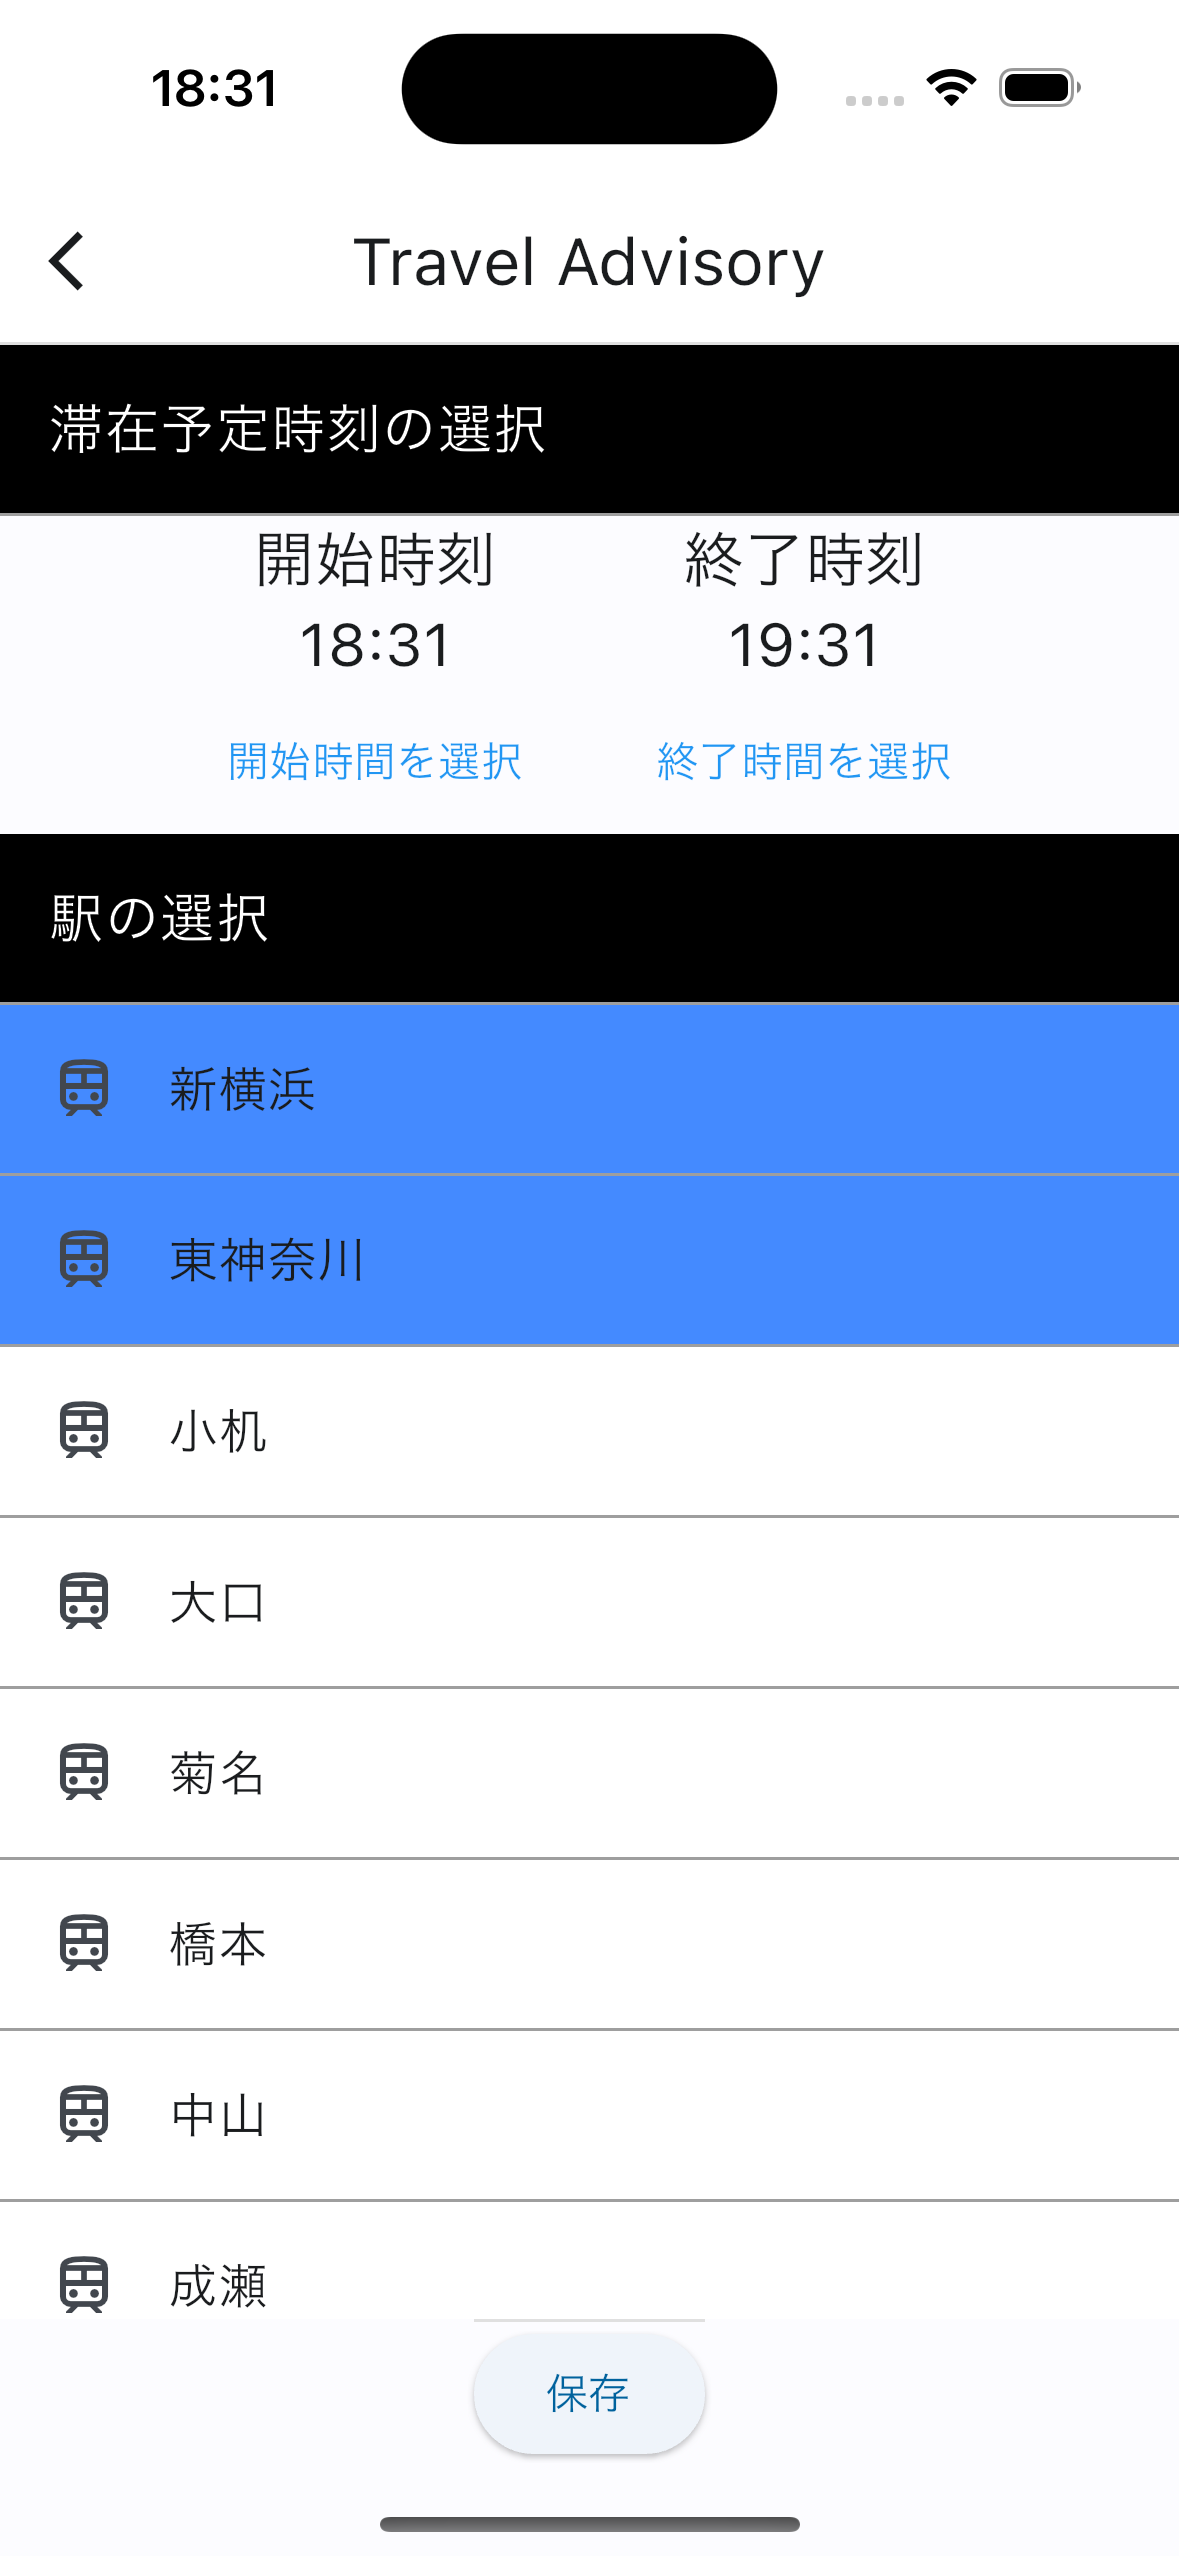
\includegraphics[height=10cm]{./fig/trans_data_save.png}
    %\vspace{-3mm}
    \caption{利用する駅を保存する画面}
    \label{fig:trans_data_save}
    %\vspace{2mm}
  \end{minipage}
\end{figure}

\subsection {通知を受け取る}
通知をタップする.
保存した旅程データがバッチ処理によって災害情報と紐付けられると,push通知が届く.
そしてホーム画面の災害注意予報一覧から注意報が出ている旅程パッケージをタップする.
なお,本アプリにおいては遠隔からの通知を受け取る仕様ではなく,ユーザがアプリを通じて通知を送信する.
本来であれば遠隔から通知を受け取るべきだが,後述する評価実験に関係のない機能であることから本実験では実装を見送った.

\begin{figure}[H]
  \begin{minipage}[b]{0.45\linewidth}
    \centering
    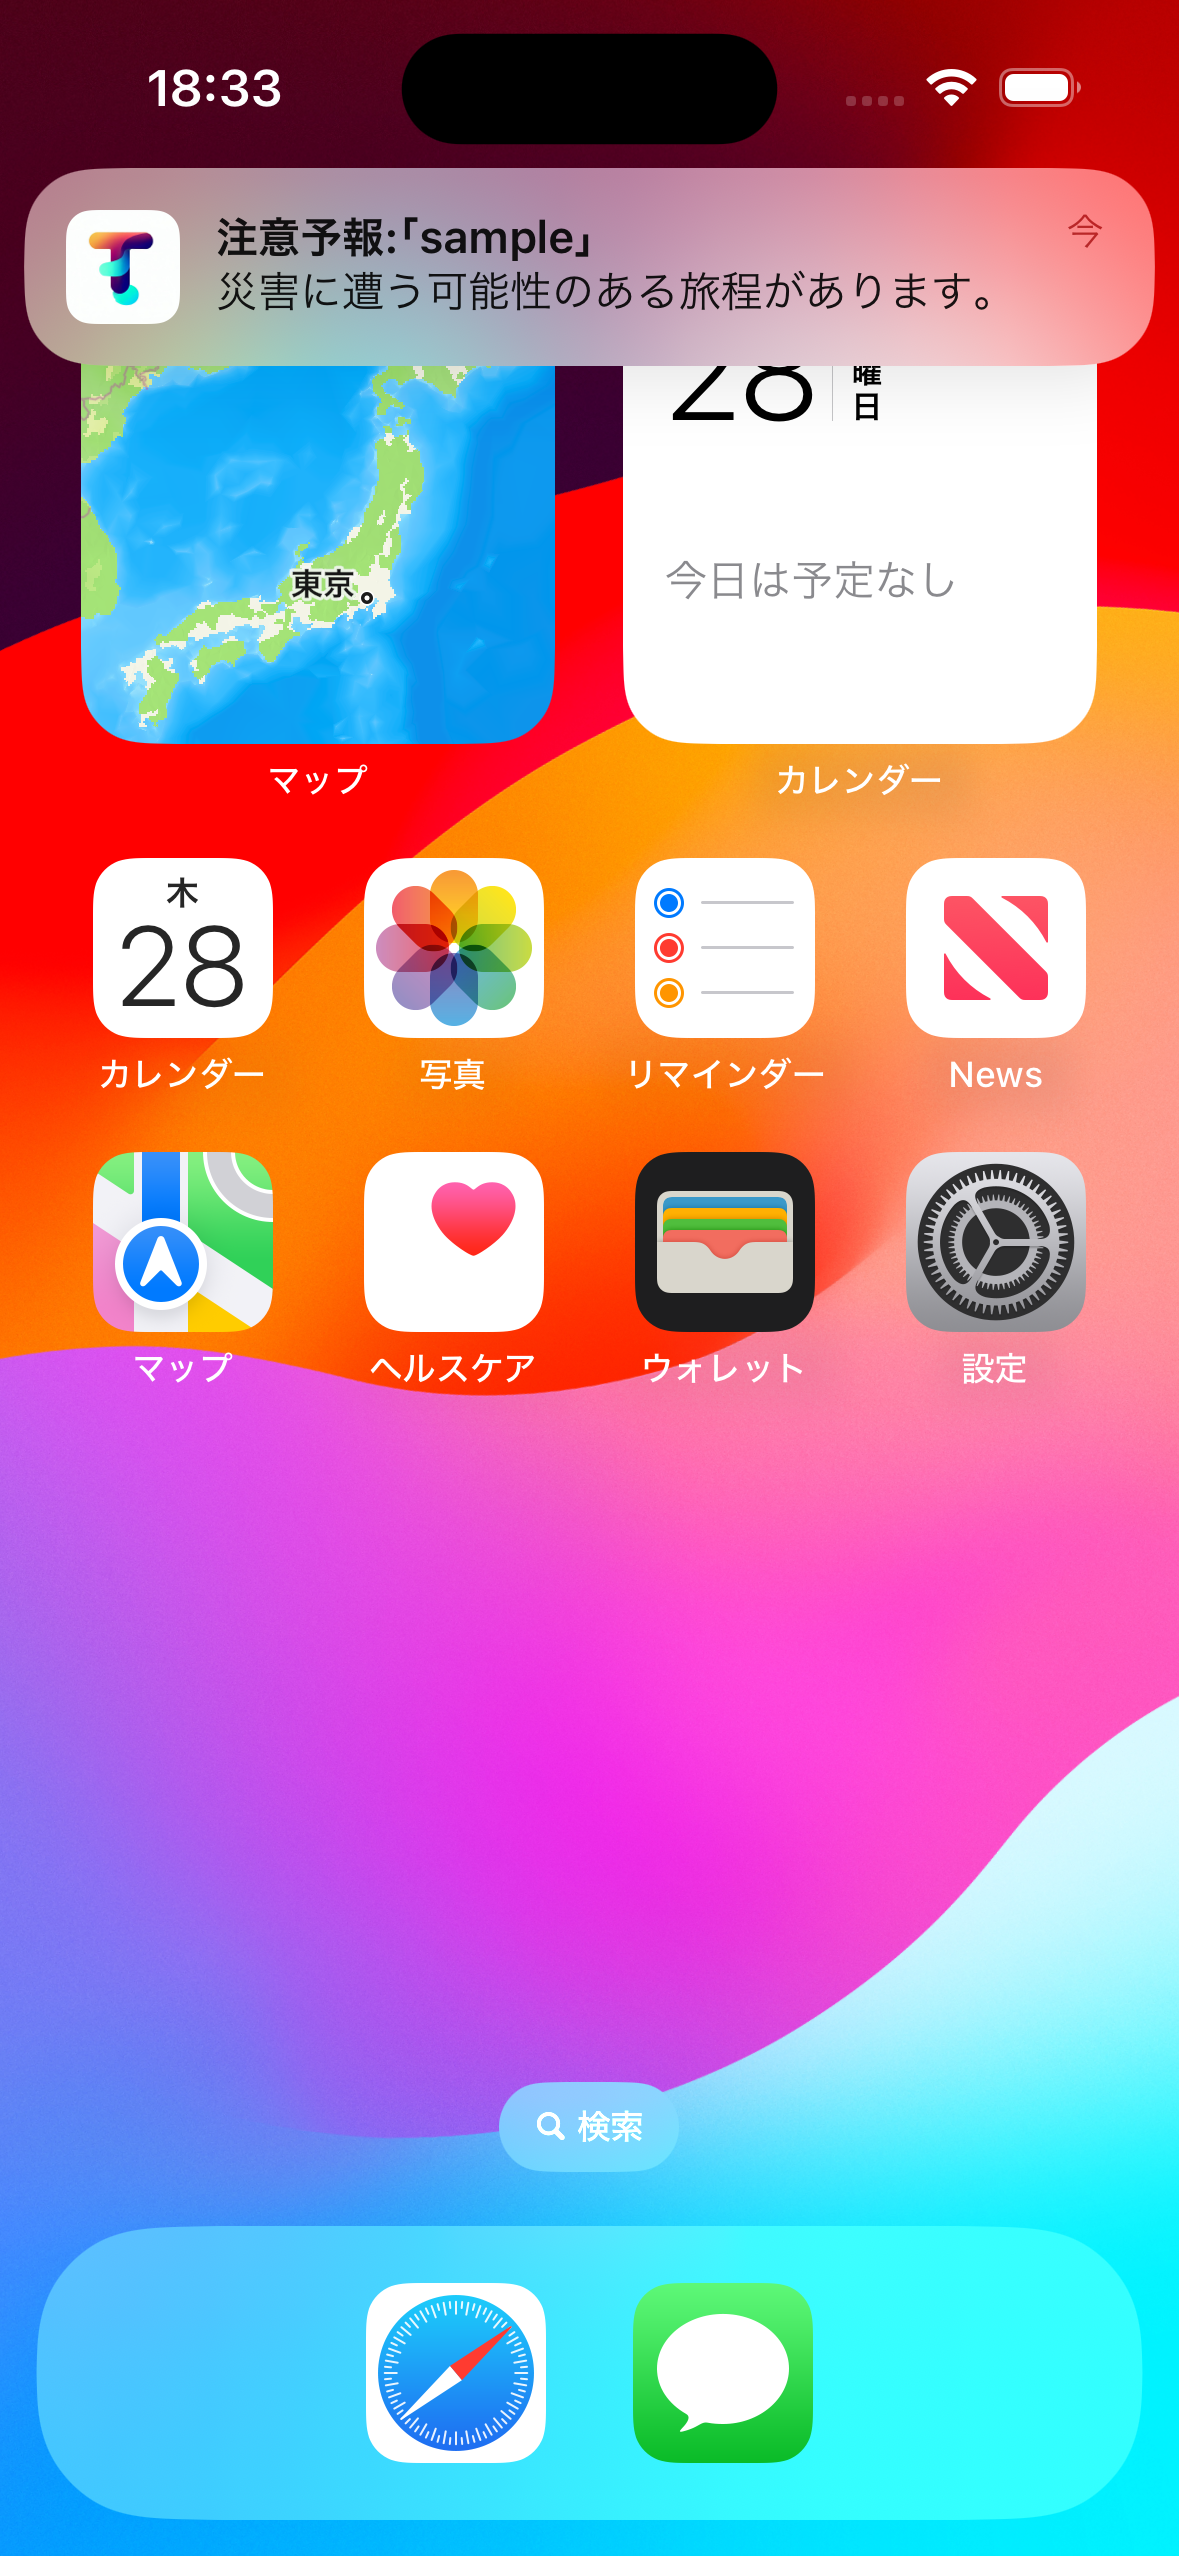
\includegraphics[height=10cm]{./fig/notion.png}
    %\vspace{-3mm}
    \caption{通知の表示}
    \label{fig:notion}
    %\vspace{2mm}
  \end{minipage}
  \begin{minipage}[b]{0.45\linewidth}
    \centering
    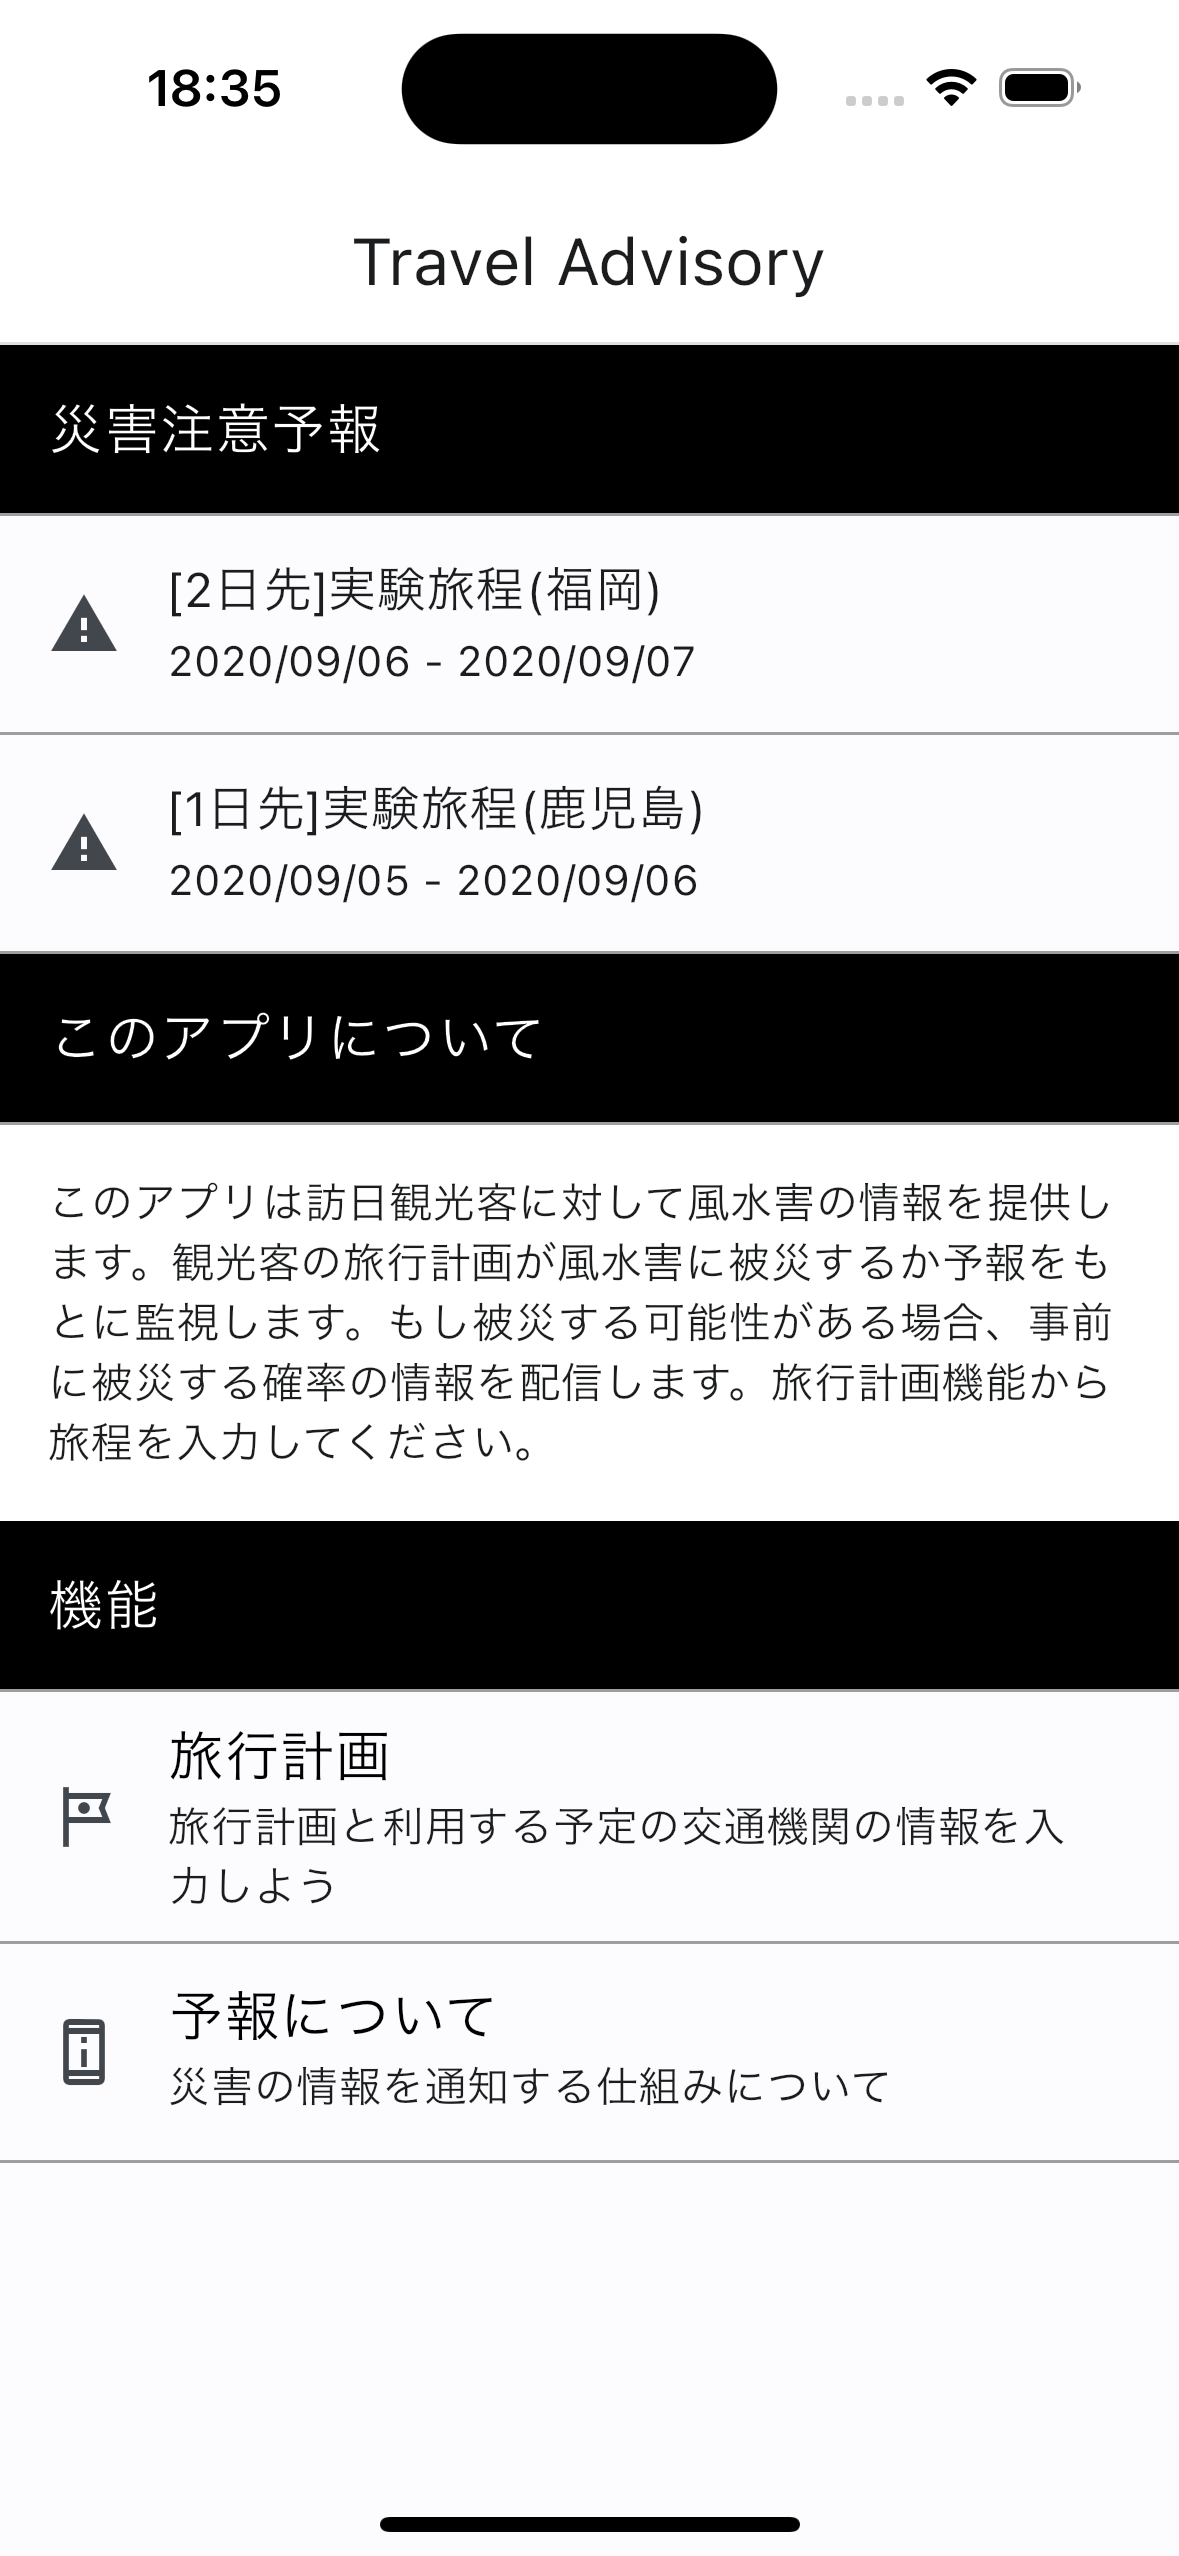
\includegraphics[height=10cm]{./fig/unormal_home_screen.png}
    %\vspace{-3mm}
    \caption{災害注意予報通知時のホーム画面}
    \label{fig:unormal_home_screen}
    %\vspace{2mm}
  \end{minipage}
\end{figure}

\subsection {災害注意予報を確認する}
選択した旅行パッケージの災害注意予報が紐付けられている旅程データの一覧を閲覧する.
一覧から旅程データを選択する.
\begin{figure}[H]
  \centering
  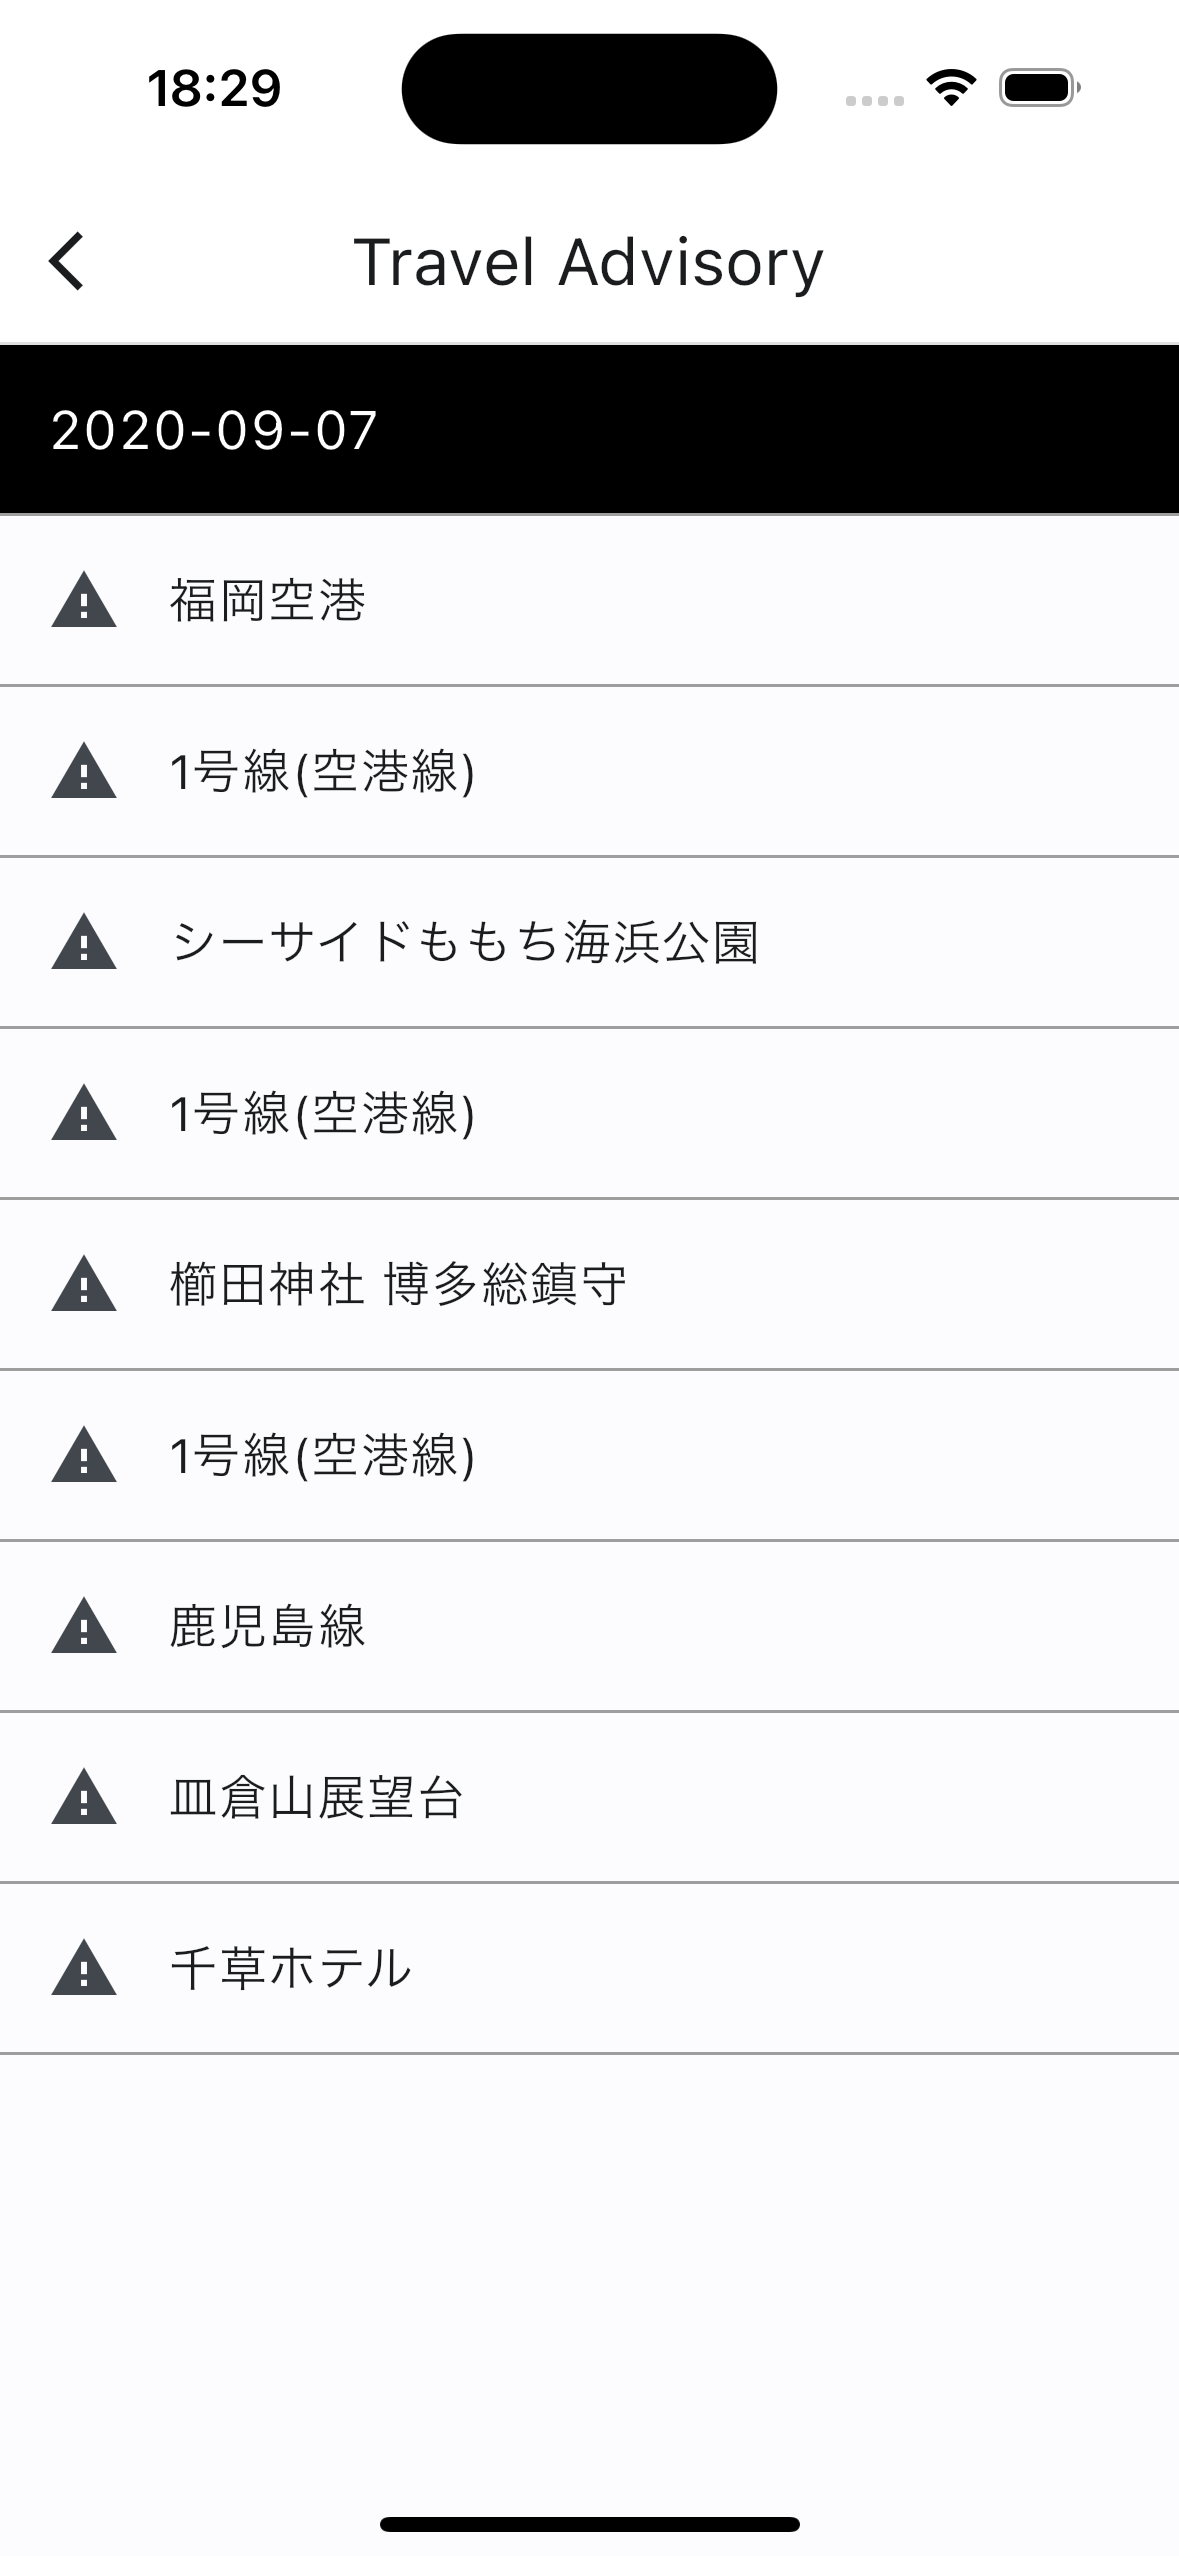
\includegraphics[height=10cm]{./fig/advisory_data_list.png}
  %\vspace{-3mm}
  \caption{災害注意予報が出ている旅程データの一覧}
  \label{fig:advisory_data_list}
  %\vspace{2mm}
\end{figure}

\subsubsection {場所データの災害注意予報}
場所データに対する災害注意予報を閲覧する.
提供される災害の種類は雨と風(風雪)である.災害の種類ごとに災害が起こる確率を提供している.
それぞれの災害のリストをタップすると,ストック情報の画面に遷移する.

\begin{figure}[H]
  \centering
  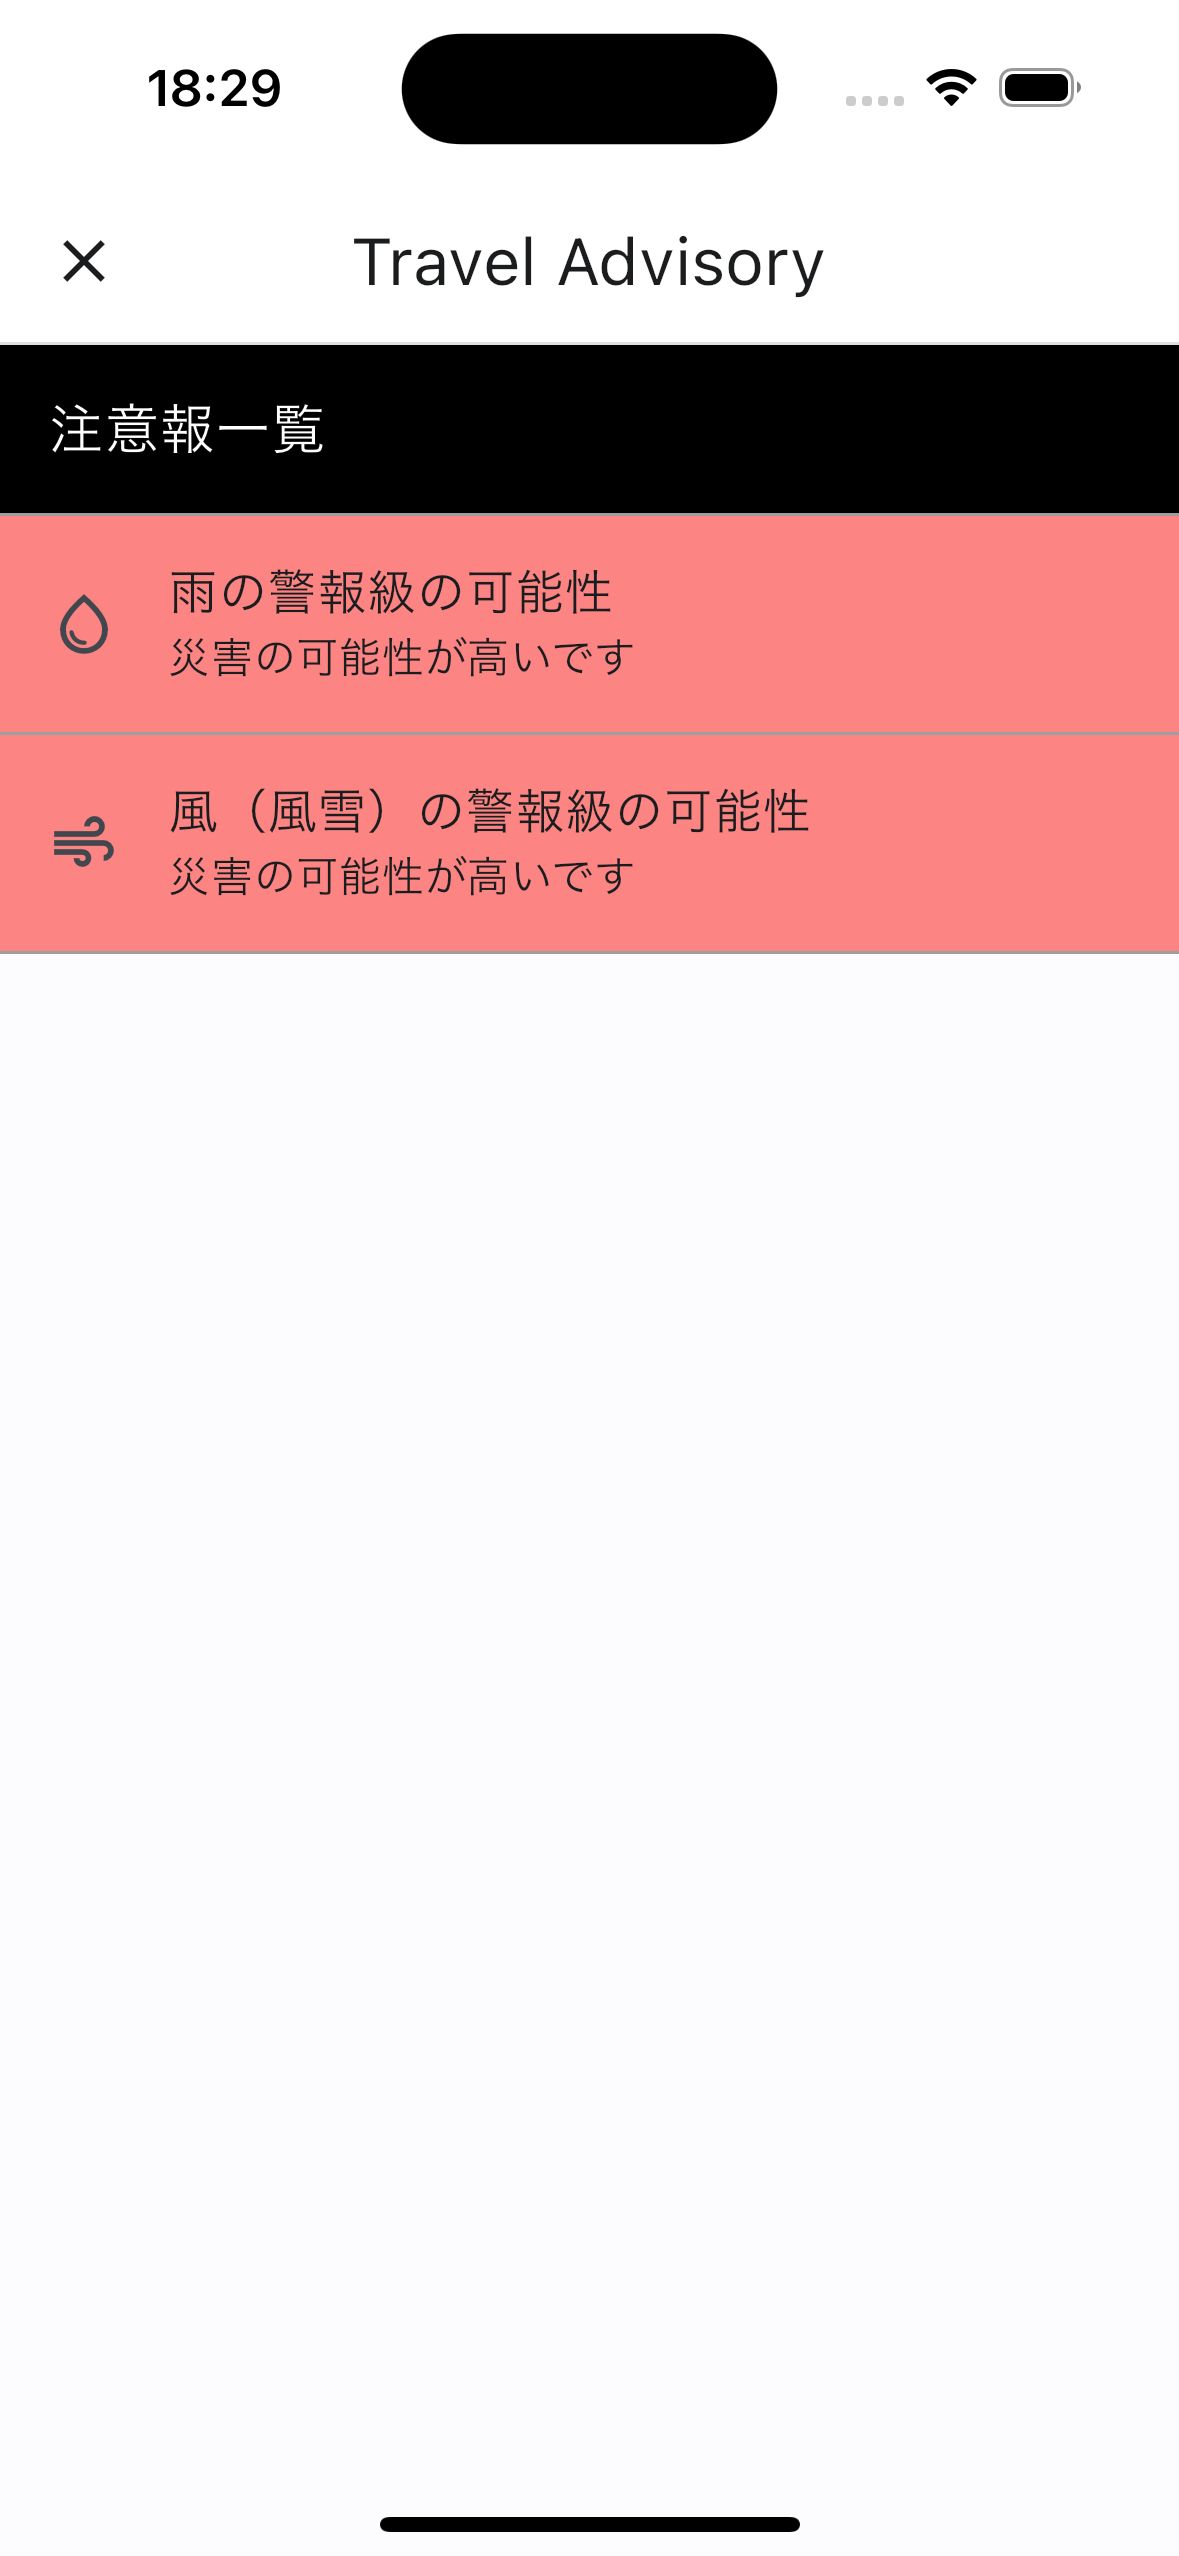
\includegraphics[height=10cm]{./fig/spot_advisory.png}
  %\vspace{-3mm}
  \caption{場所データの災害注意予報画面}
  \label{fig:spot_advisory}
  %\vspace{2mm}
\end{figure}

\subsubsection {交通データの災害注意予報}
交通データに対する災害注意予報を閲覧する.
交通データにおいては,場所データと同じように駅データごとに災害注意予報が提供される.
各駅に対して災害の発生する可能性を運休する可能性として情報を提供している.
さらに,ページ下部には災害時に起こる交通機関の運休の現象や計画運休の現象についての説明がある.

\begin{figure}[H]
  \begin{minipage}[b]{0.45\linewidth}
    \centering
    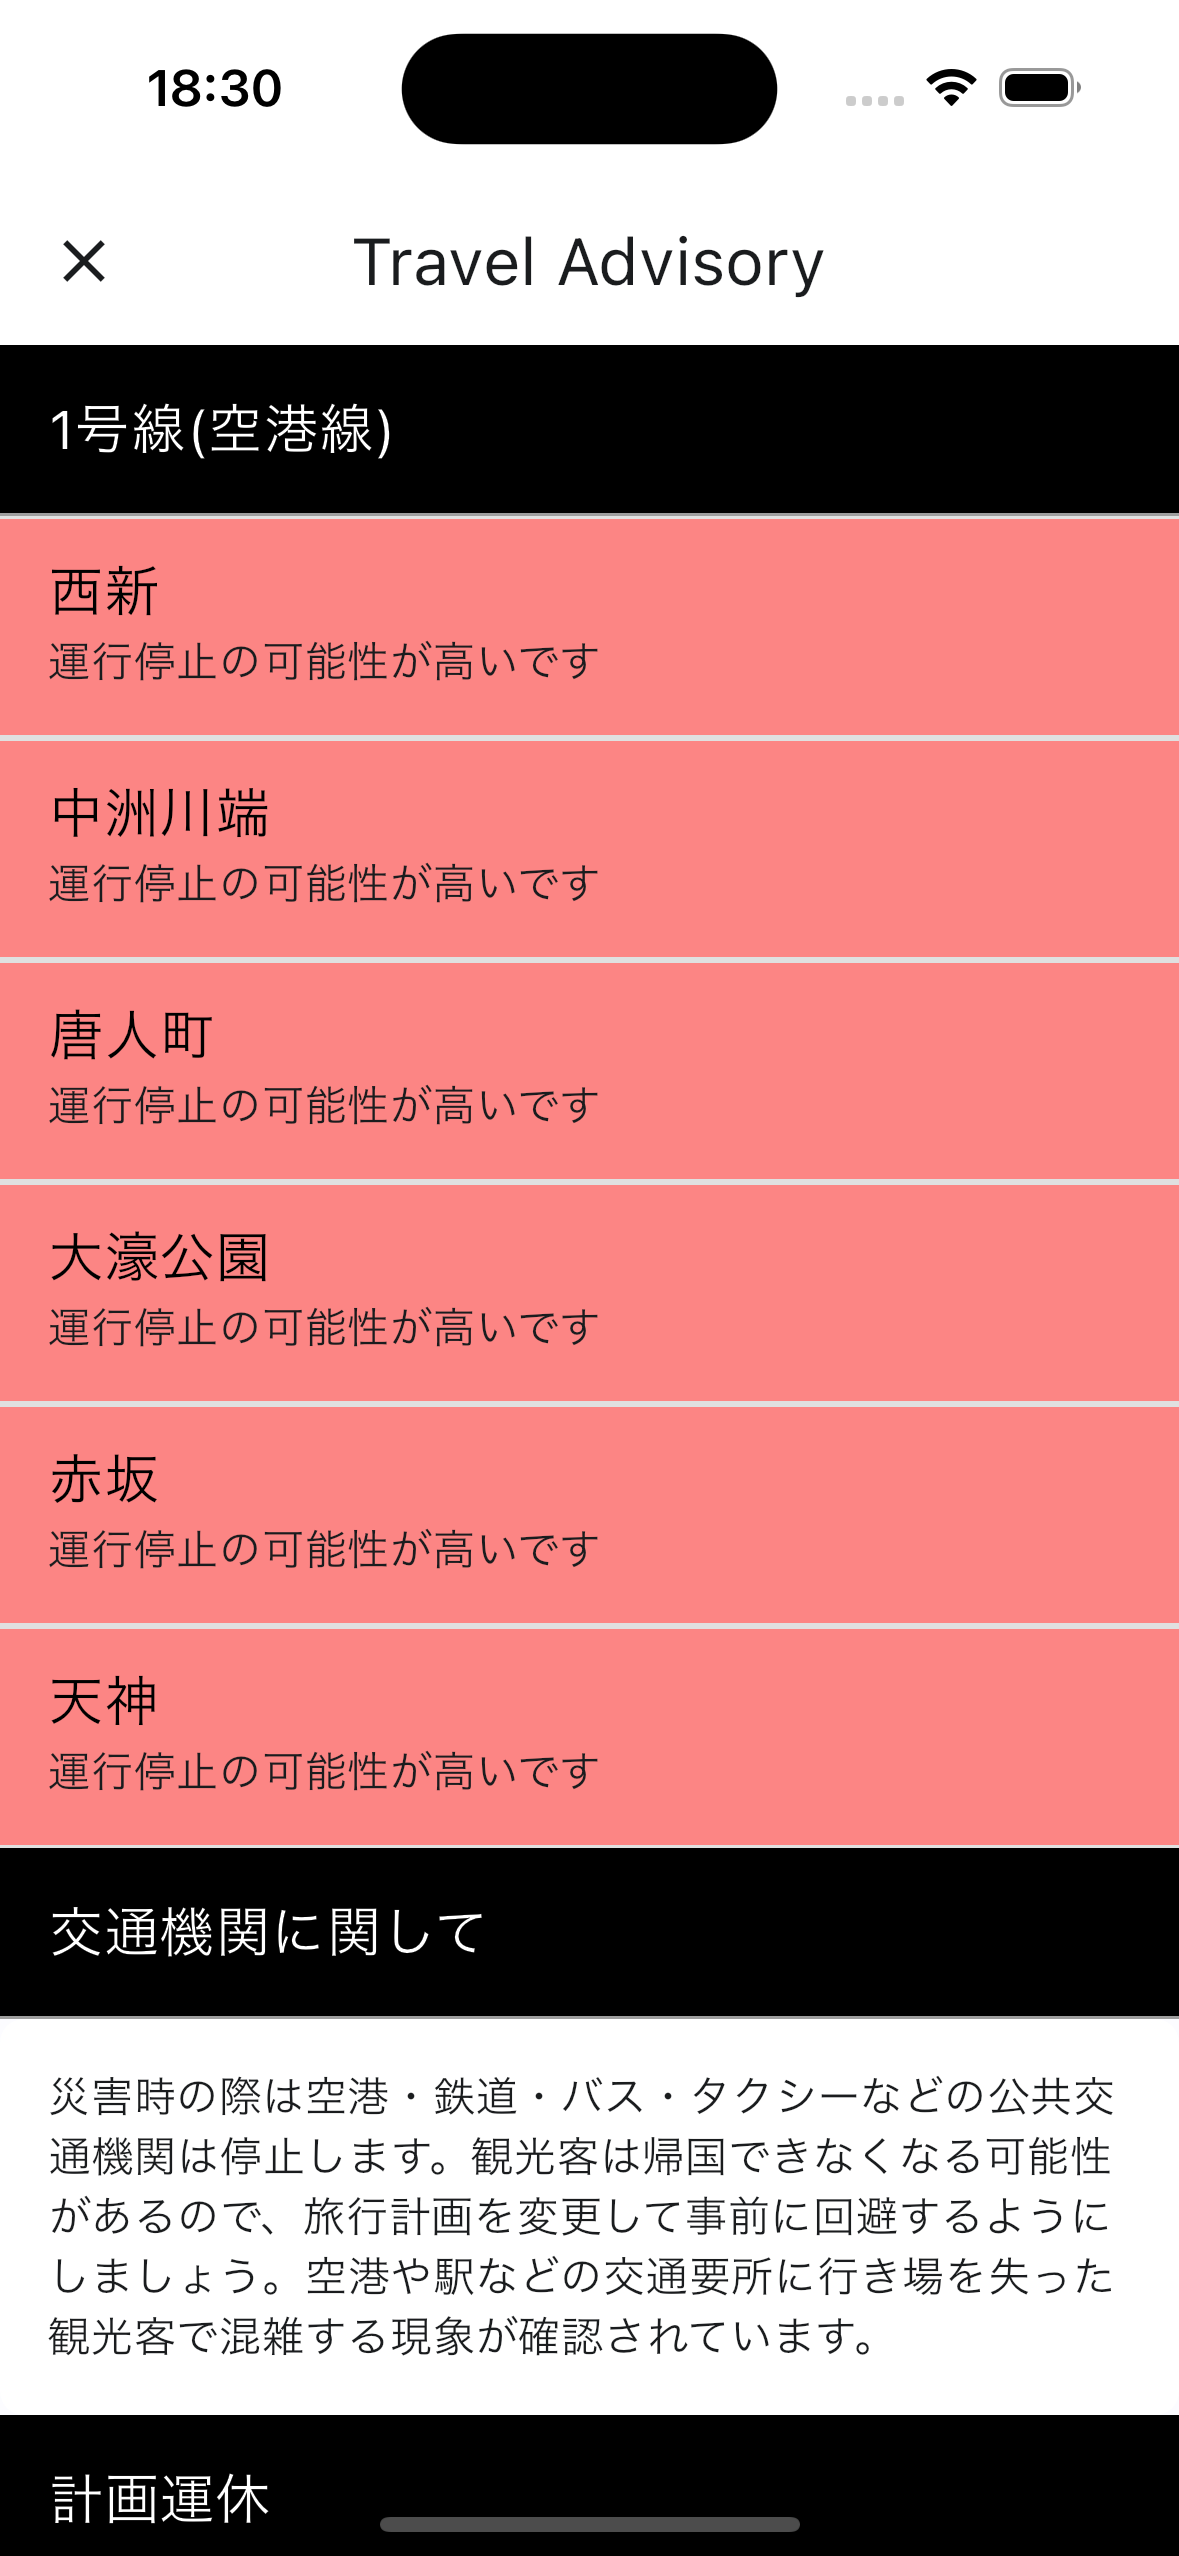
\includegraphics[height=10cm]{./fig/trans_advisory_1.png}
    %\vspace{-3mm}
    \caption{交通データの災害注意予報画面1}
    \label{fig:trans_advisory_1}
    %\vspace{2mm}
  \end{minipage}
  \begin{minipage}[b]{0.45\linewidth}
    \centering
    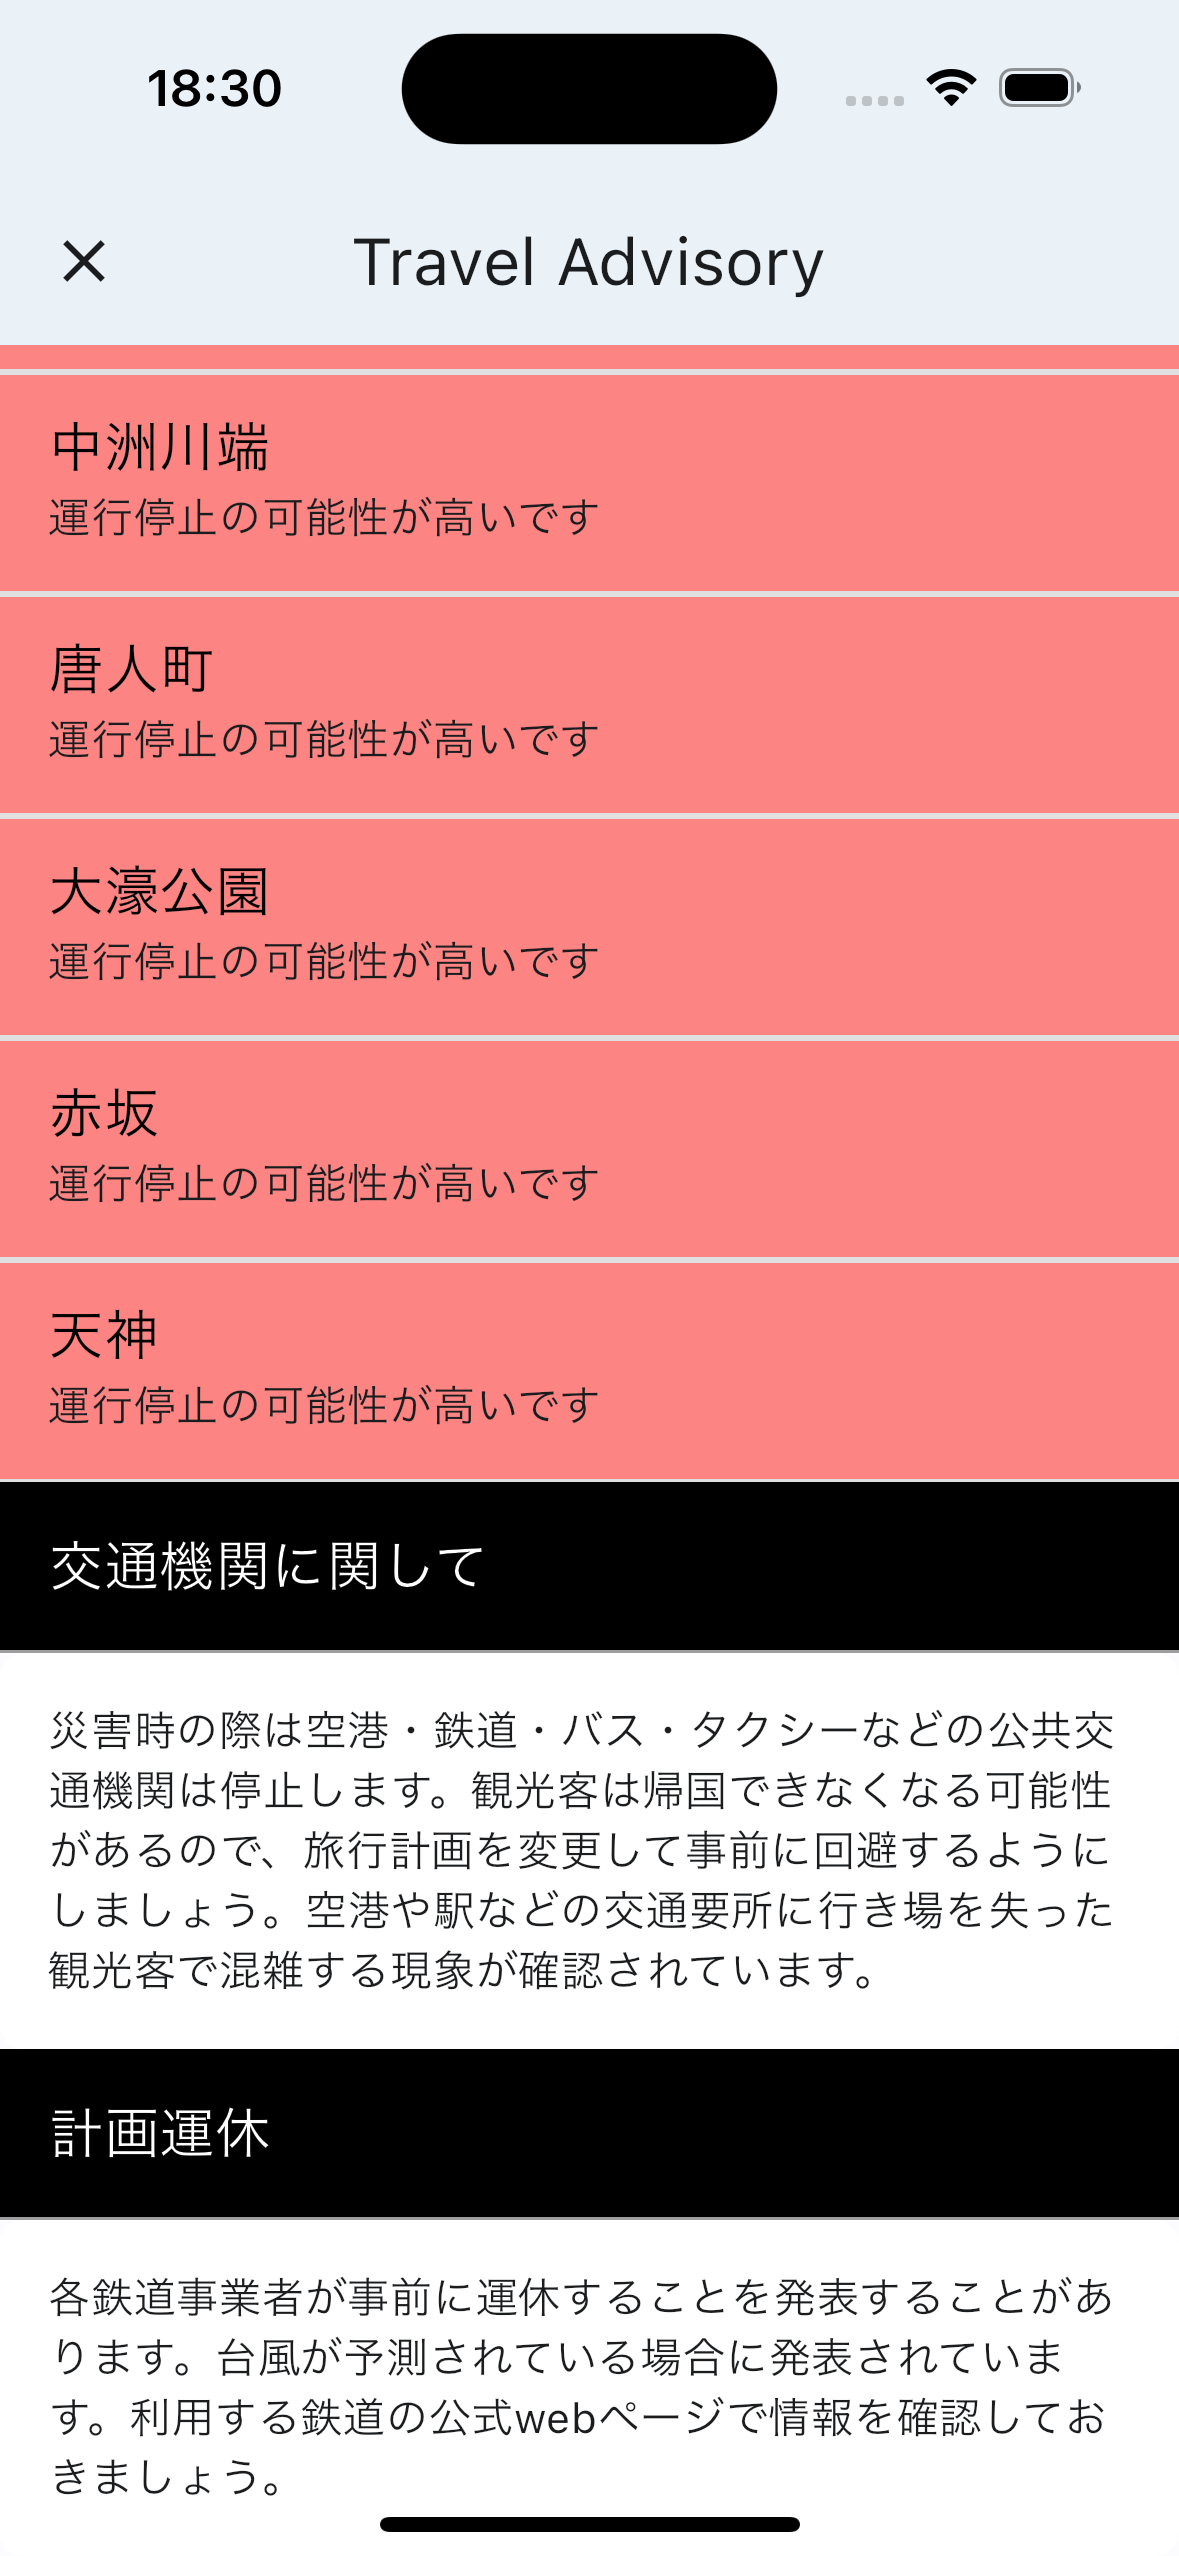
\includegraphics[height=10cm]{./fig/trans_advisory_2.png}
    %\vspace{-3mm}
    \caption{交通データの災害注意予報画面2}
    \label{fig:trans_advisory_2}
    %\vspace{2mm}
  \end{minipage}
\end{figure}

\subsection {ストック情報を確認する}
災害のストック情報を閲覧する.
ストック情報は雨と風(風雪)の2種類の災害の情報である.

\subsubsection {雨の災害の情報}
日本における雨に関する災害についての説明が記載されている.
雨に関する災害とは大雨そのものの現象以外に洪水と土砂災害のことである.
各災害についての説明とそれに対する対策喚起の情報が載っている.

\begin{figure}[H]
  \begin{minipage}[b]{0.45\linewidth}
    \centering
    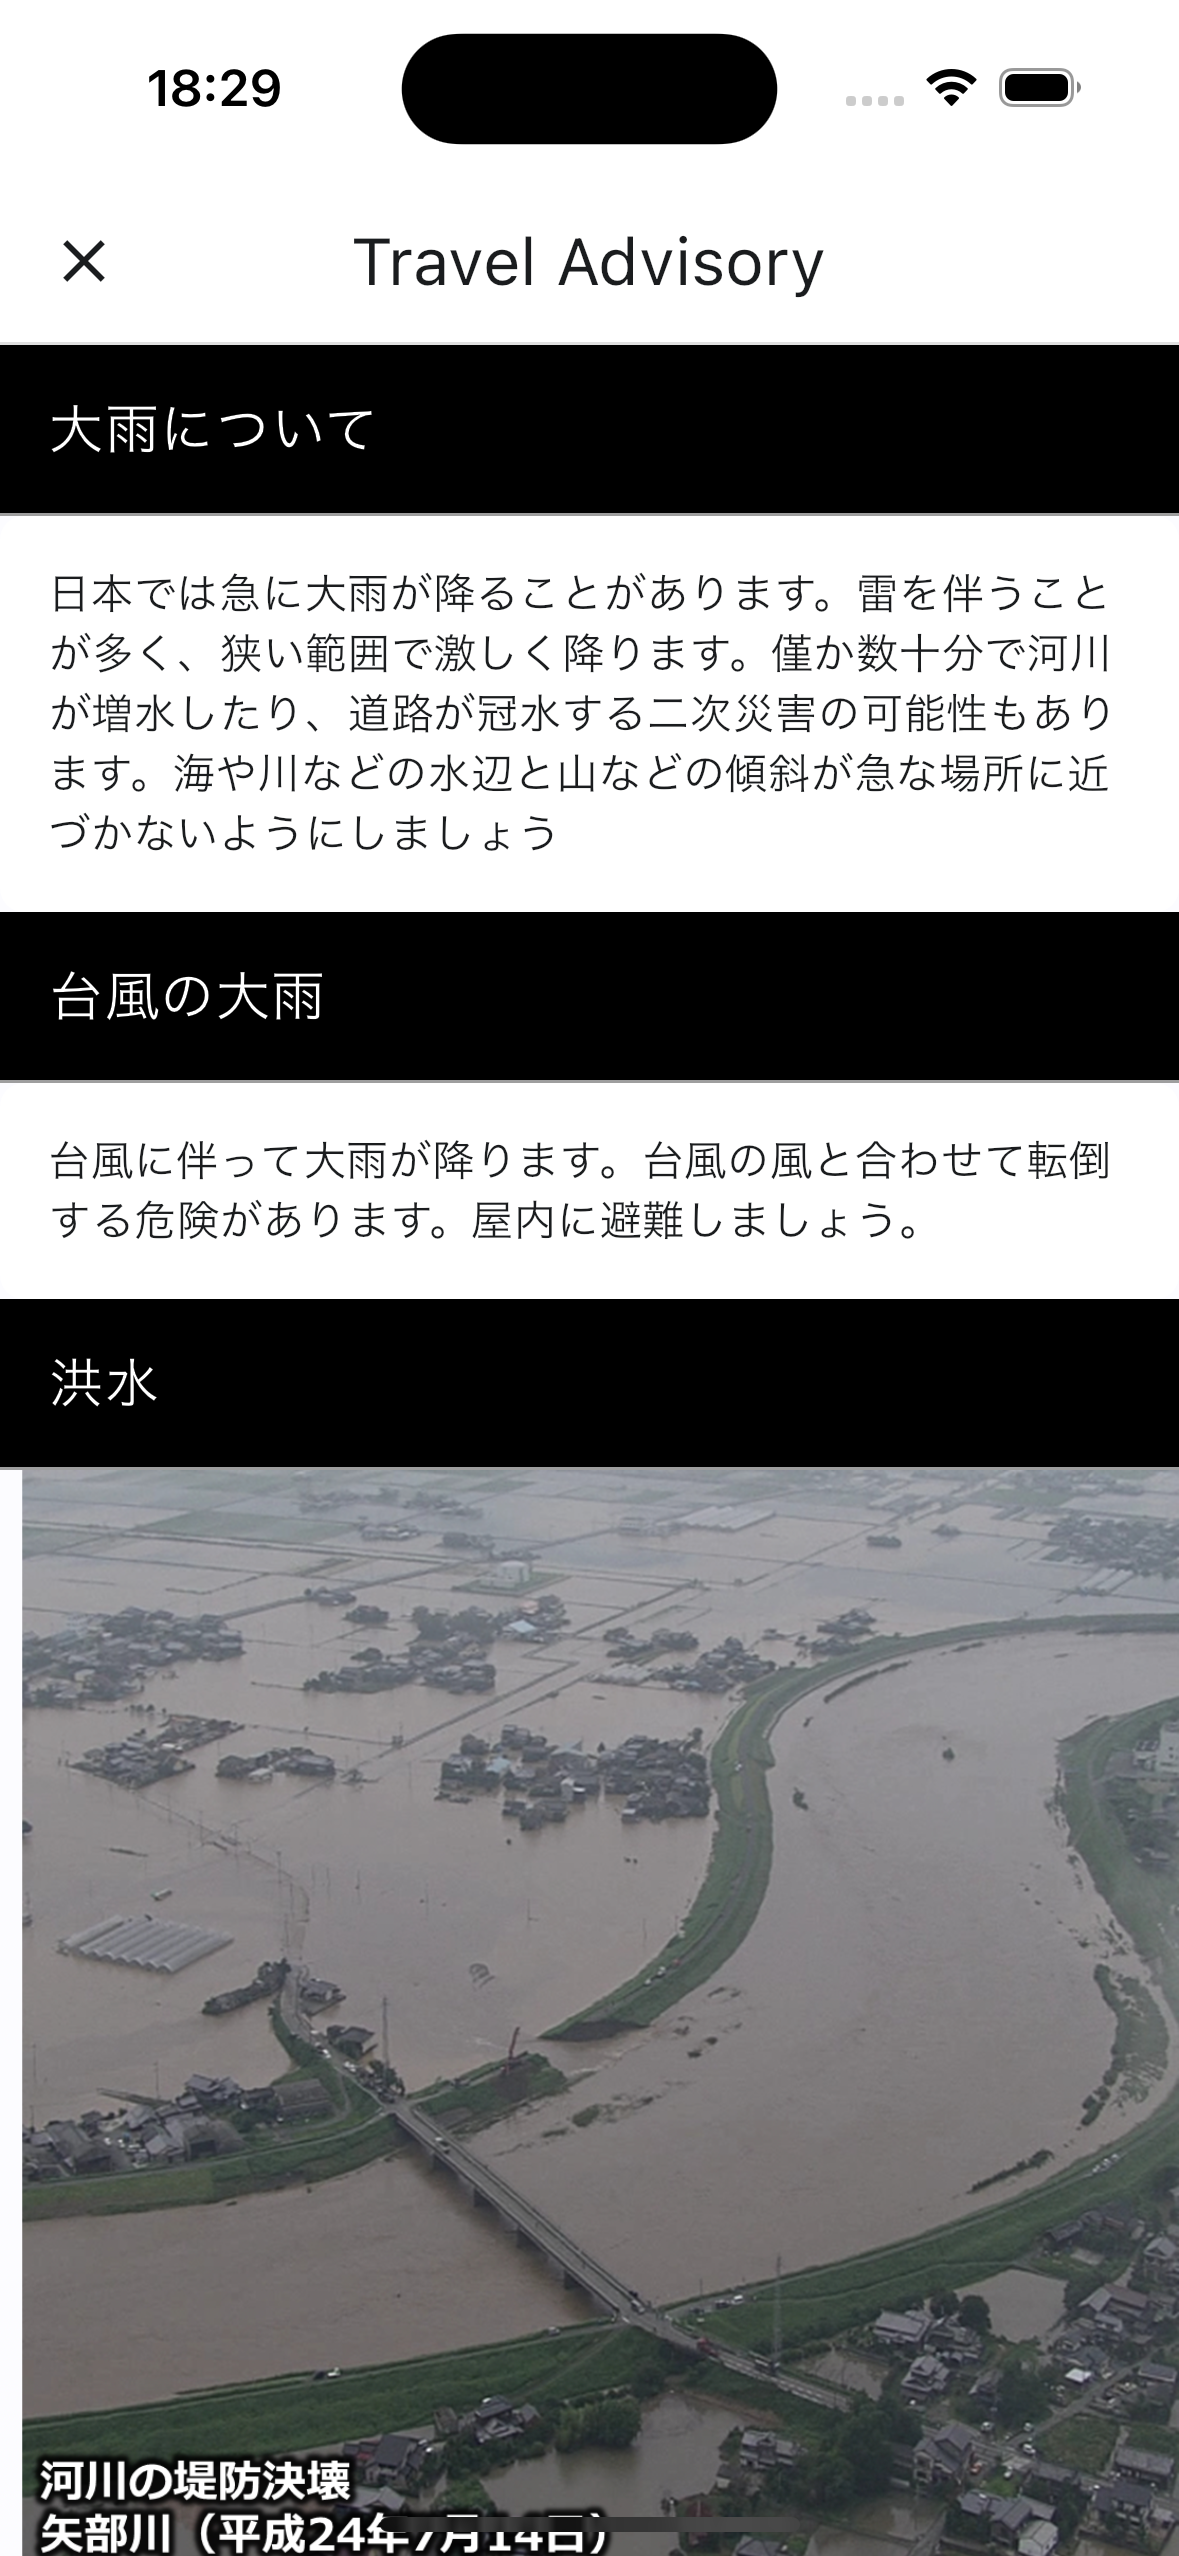
\includegraphics[height=10cm]{./fig/rain_stock_1.png}
    %\vspace{-3mm}
    \caption{雨のストック情報提供画面1}
    \label{fig:rain_stock_1}
    %\vspace{2mm}
  \end{minipage}
  \begin{minipage}[b]{0.45\linewidth}
    \centering
    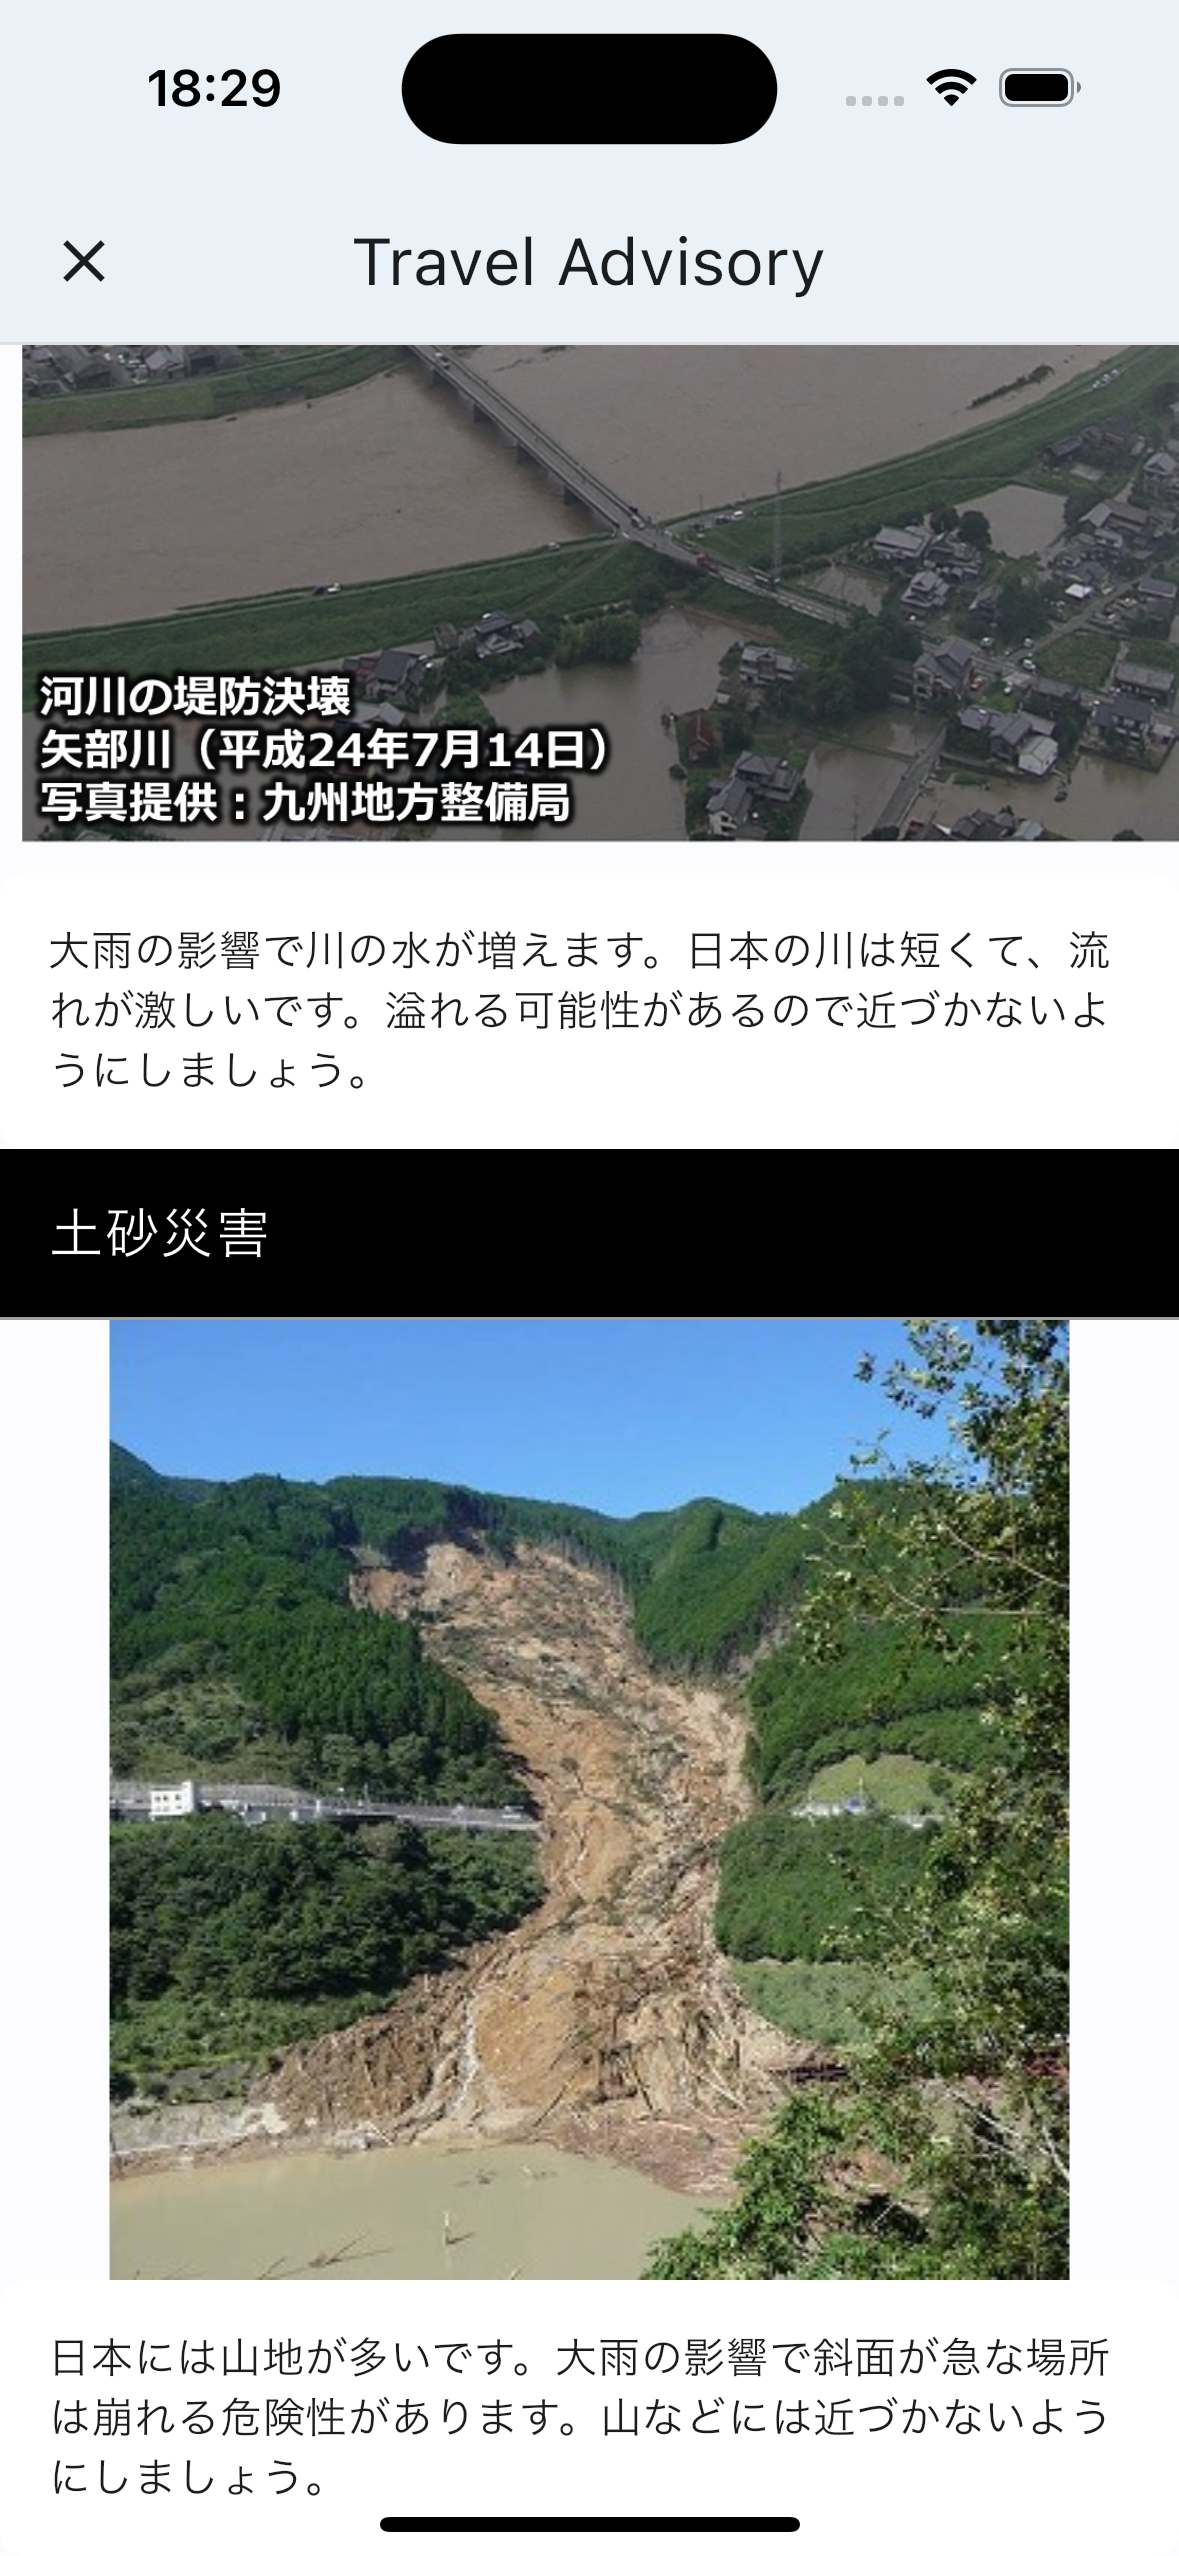
\includegraphics[height=10cm]{./fig/rain_stock_2.png}
    %\vspace{-3mm}
    \caption{雨のストック情報提供画面2}
    \label{fig:rain_stock_2}
    %\vspace{2mm}
  \end{minipage}
\end{figure}

\subsubsection {風の災害の情報}
日本における風に関する災害についての説明が記載されている.
具体的には台風と高潮,暴風についてである.
各災害についての説明とそれに対する対策喚起の情報が載っている.

\begin{figure}[H]
  \begin{minipage}[b]{0.45\linewidth}
    \centering
    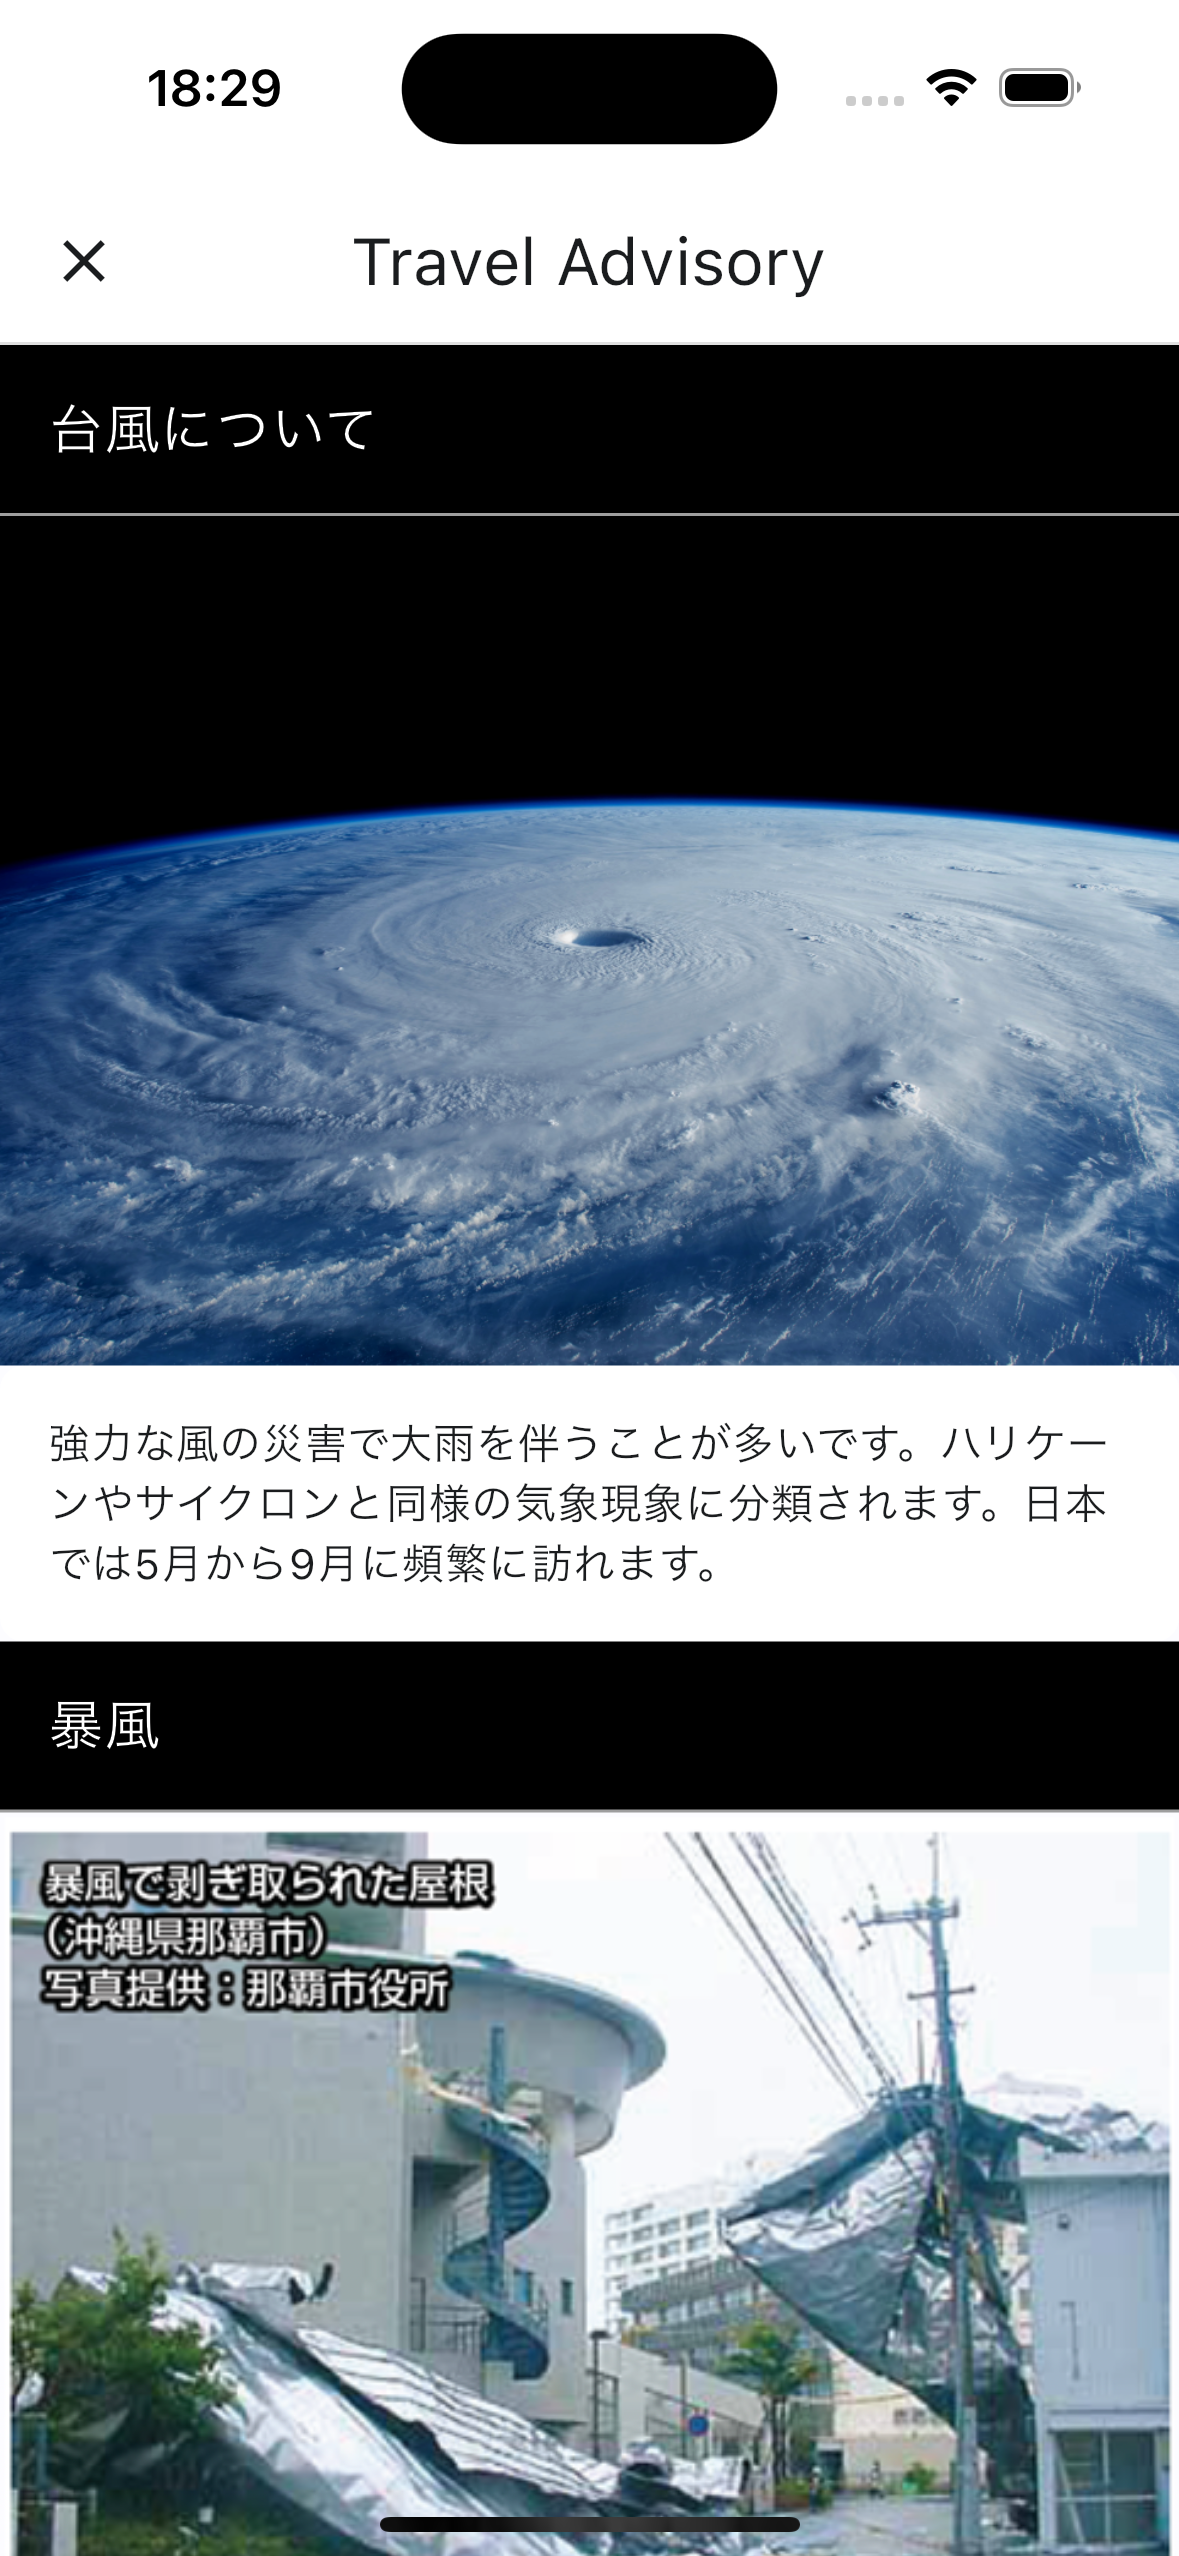
\includegraphics[height=10cm]{./fig/wind_stock_1.png}
    %\vspace{-3mm}
    \caption{風のストック情報提供画面1}
    \label{fig:rain_stock_1}
    %\vspace{2mm}
  \end{minipage}
  \begin{minipage}[b]{0.45\linewidth}
    \centering
    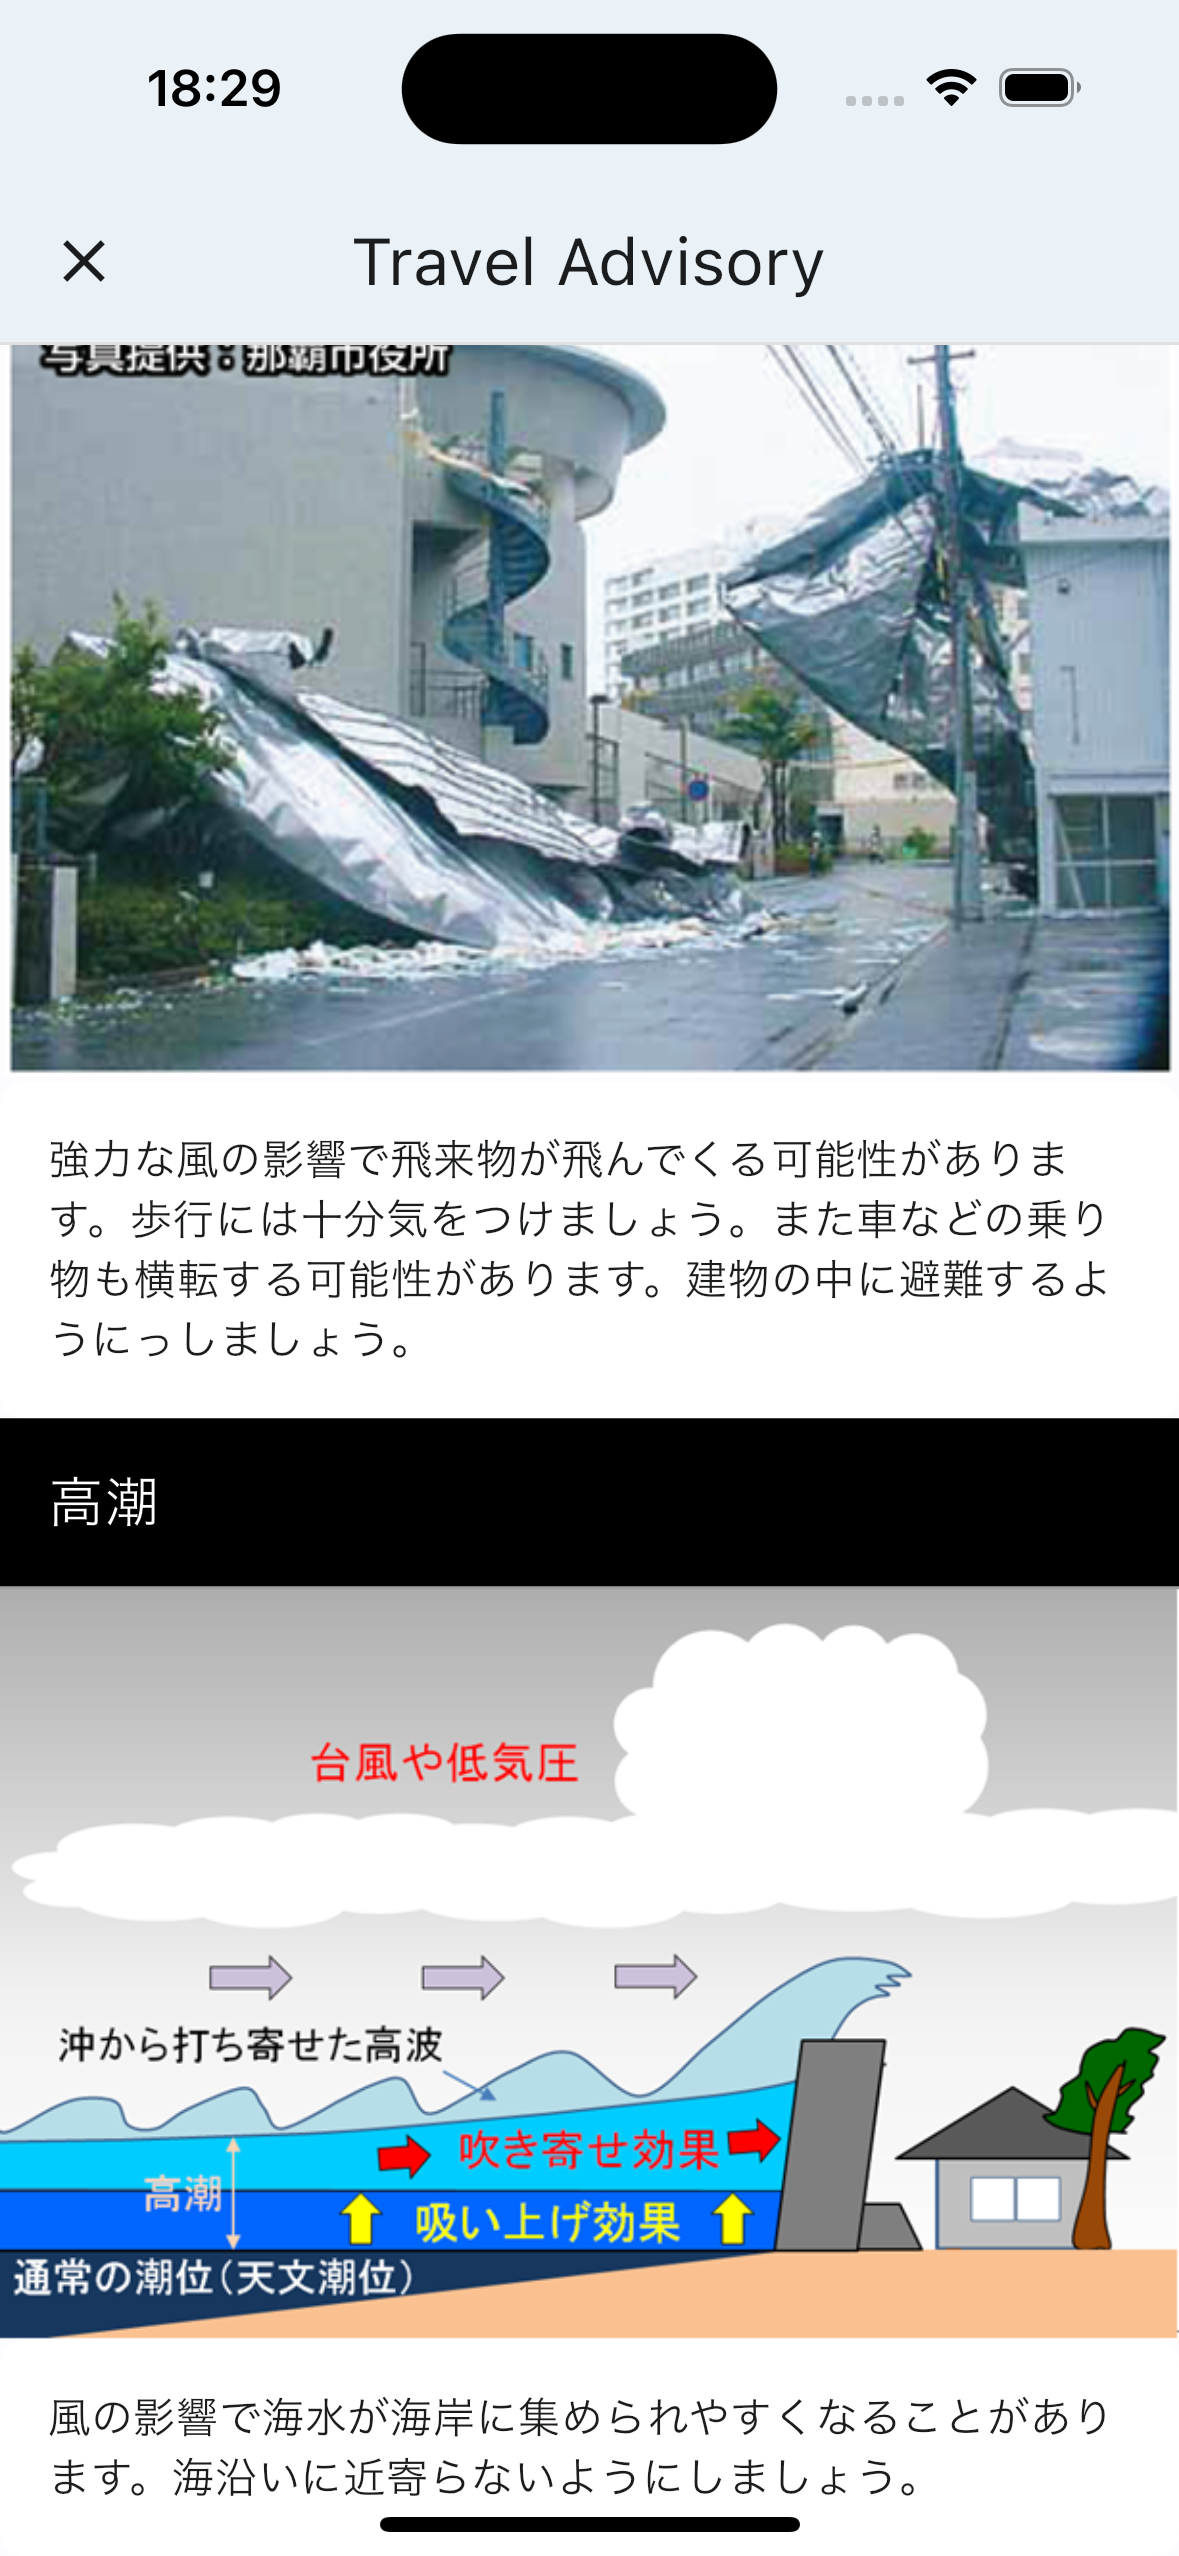
\includegraphics[height=10cm]{./fig/wind_stock_2.png}
    %\vspace{-3mm}
    \caption{風のストック情報提供画面2}
    \label{fig:rain_stock_2}
    %\vspace{2mm}
  \end{minipage}
\end{figure}

% \begin{figure}[H]
%   \centering
%   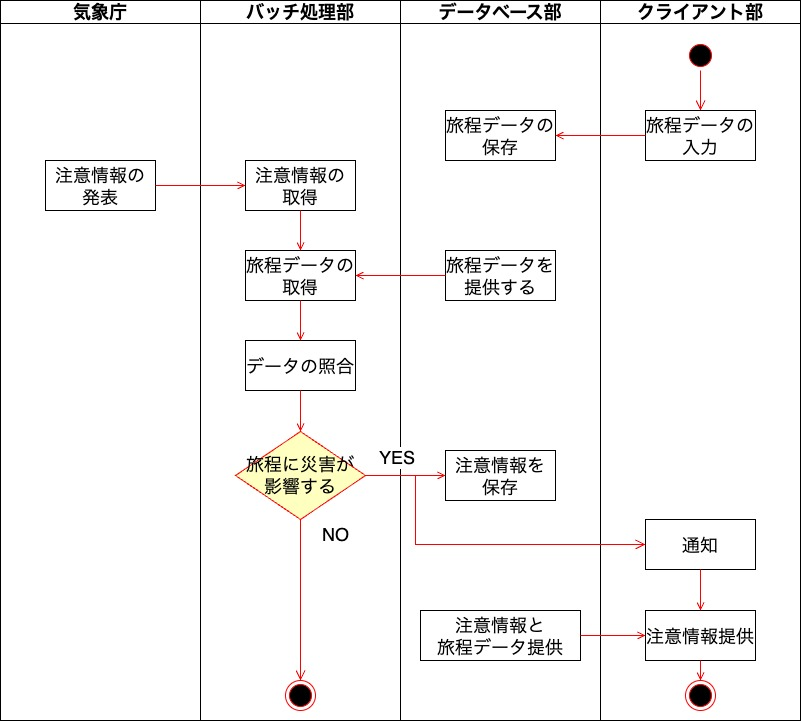
\includegraphics[height=8cm]{figure32.jpg}
%   %\vspace{-3mm}
%   \caption{場所データの注意情報提供画面の図}
%   \label{fig:activity}
%   %\vspace{2mm}
% \end{figure}

% \subsection {公共交通データの注意情報提供画面の図}

% \begin{figure}[H]
%   \centering
%   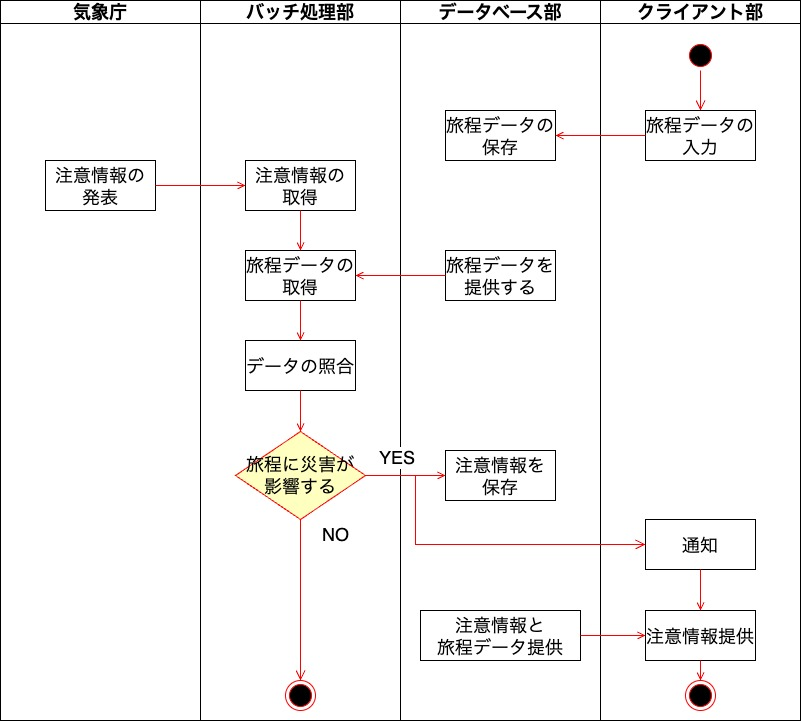
\includegraphics[height=8cm]{figure32.jpg}
%   %\vspace{-3mm}
%   \caption{公共交通データの注意情報提供画面の図}
%   \label{fig:activity}
%   %\vspace{2mm}
% \end{figure}

% \subsection {大雨に関するストック情報の提供画面の図}

% \begin{figure}[H]
%   \centering
%   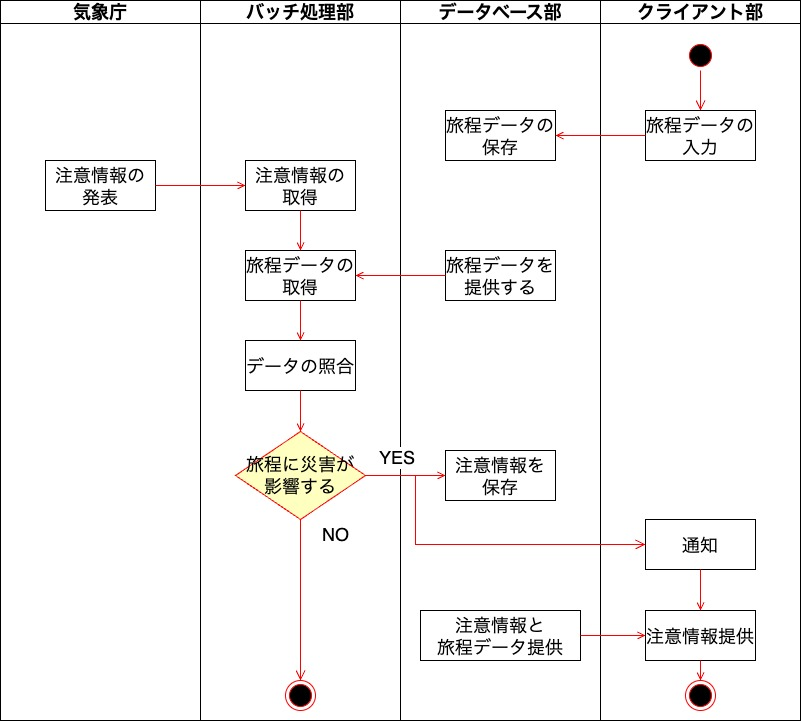
\includegraphics[height=8cm]{figure32.jpg}
%   %\vspace{-3mm}
%   \caption{大雨に関するストック情報の提供画面の図}
%   \label{fig:activity}
%   %\vspace{2mm}
% \end{figure}

% \subsection {風に関するストック情報の提供画面}

% \begin{figure}[H]
%   \centering
%   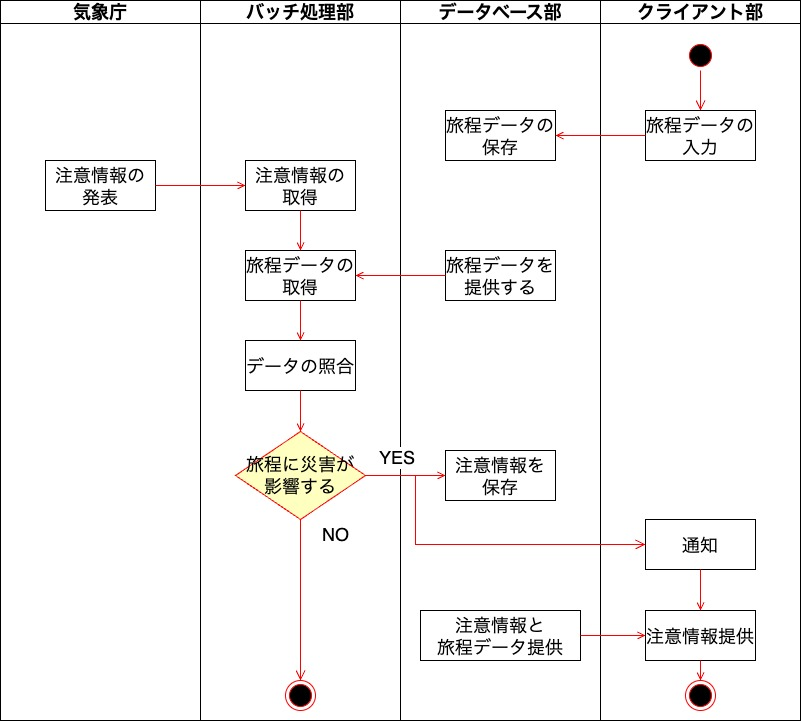
\includegraphics[height=8cm]{figure32.jpg}
%   %\vspace{-3mm}
%   \caption{風に関するストック情報の提供画面の図}
%   \label{fig:activity}
%   %\vspace{2mm}
% \end{figure}
%
\end{document}